% !Mode:: "TeX:UTF-8"
\part{数学基础与算法}
\label{part:math_learning}

\newpage

AI最近变得非常流行了,但它的历史已经有六十多年。在1956年的达特茅斯会议,首次提出了AI的概念,
而在一年后,\emph{Rosenblatt}就提出了\emph{感知机}(perceptron)模型。


\begin{figure}[!htb]
\newcounter{TempEqCnt}
\setcounter{TempEqCnt}{\value{chapter}}
\setcounter{chapter}{0} 
\centering
\begin{tikzpicture}[node distance=1cm]
%定义流程图具体形状
\node[perceptron](circle){$\Sigma$};
%连接具体形状
\node[left of=circle,xshift=-2cm,yshift=1cm,draw=none,fill=none](x1){x1};
\node[left of=circle,xshift=-2cm, draw=none,fill=none](x2){x2};
\node[left of=circle,xshift=-2cm,yshift=-1cm, draw=none,fill=none](x3){x3};
\node[right of=circle,xshift=2cm,draw=none,fill=none](output){output};
\draw [arrow](x1) -- (circle);
\draw [arrow](x2) -- (circle);
\draw [arrow](x3) -- (circle);
\draw [arrow](circle)--(output);
\end{tikzpicture}
\caption{感知机}
\label{fig:part2_math_perceptron}
\end{figure}
\setcounter{chapter}{\value{TempEqCnt}} 

如上\figref{fig:part2_math_perceptron},\emph{感知机}就是二分类的线性分类模型,其输入为样本的特征向量,输出为样本的类别,取+1和-1二值。即通过某样本的特征,就可以准确判断该样本属于哪一类。顾名思义,感知机能够解决的问题首先要求特征空间是线性可分的,再者是二分类,即将样本分为{+1, -1}两类。


使用\emph{感知机}可轻松解决异、或、非的问题,却存在一个致命缺陷:无法解决异或问题。导致\emph{AI}进入第一个衰退期,直到19世纪八十年代,才逐渐复苏。
1984年,Hiton 教授提出\emph{Boltzman}机模型。到1986年 Kumelhart 等人提出\emph{误差反向传播}(Back Propagation)算法,简称 BP 网络。然而90年中期\emph{支持向量机}(Support Vector Machines,SVM)强势登场,全方位碾压NN。SVM具有 1)\emph{高效},可以快速训练;2)\emph{无需调参},没有梯度消失问题;3)\emph{高效泛化,全局最优解},不存在过拟合问题。几乎全方位的碾压NN,NN也再次被打入冷宫。


目前,BP网络已成为广泛使用的网络。1987年至今为发展期,神经网络受到各个国家的重视,纷纷展开研究,形成神经网络发展的另一个高潮。
人工智能是一个将数学、算法和工程相结合的学科,包含微积分、概率论、统计学等数学知识。
本章将为大家简要介绍人工智相关的数学基础理论。


% \chapter{数学基础-DEMO}
\label{chap:math_regression}

\gls{AI}实在是一个多学科综合性应用,涉及到的理论不仅多而且深。限于笔者知识水平以及篇幅要求,不会对此进行长篇巨幅地解释。


\section{向量运算}
单独的一个数字,称为\emph{标量}(scalar),而向量通常用数组的形式表示。一个\emph{向量}就是一列(行)数字:
\begin{equation}
x=[x_1 x_2 \dots x_n],
x=\left[\begin{array}{c} x_1\\x_2\\\dots\\x_n\end{array}\right]
\label{part2_vector_form}
\end{equation}
\ \\
向量是一种带方向指示性的量,代表空间中的一个点。一维向量$\vec{a}=\left[4\right]$代表a点在原点右侧距离为4的位置。
而二维向量$\vec{b}=\left[3\ 4\right]$就代表了在第一象限坐标(3,4)有一个点b。所以,向量是一个方向性的偏移量。
\emph{向量}可以在坐标系中自由平移,选定一个起点就确定了它的终点。

\begin{center} \begin{tikzpicture}
\node[circle,draw,black,scale=0.2] (A) at (1,2) {};
\node[circle,draw,black,scale=0.2] (B) at (3,4) {};
\draw[arrow]
    (A)node[below]{A起点}--(B)node[above]{B终点};
\end{tikzpicture}\end{center} 

向量支持的运算有\emph{内积}(点乘)和\emph{外积}(叉乘)运算,以及加减运算。
向量A、B的运算过程,设$\vec{A} = (a1,  a2,  a3), \vec{B} = (b1,  b2,  b3)$

\begin{itemize}
\item[1.] 点乘,结果是一个标量:$A \cdot B = a1*b1 + a2*b2 + a3*b3$
\item[2.] 叉乘,结果还是个向量:$A \times B = (a2*b3 - a3*b2, a3*b1 - a1*b3, a1*b2 - a2*b1)$
\item[3.] 标量,用于每一个元素:$A + 2 = (a1+2, a2+2, a3+2)$
\end{itemize}

\noindent
通常使用\emph{数组}来表示向量,但这样扩展性不够好。咱们使用Java面向对象的方法,把数组和函数封装进一个向量类型里面去。定义一个Vector类,如\figref{fig:part2_math_vector}:

\begin{figure}[!htb]
\begin{center}\begin{tikzpicture}
\umlclass[y=-3]{InVector}{
    array : int[] 
}{
    add(v : InVector) : InVector \\
    sub(v : InVector) : InVector \\
    dot(v : InVector) : int \\
    cross(v : InVector) : IntVector
}
\label{fig:part2_math_vector}
\end{tikzpicture}\end{center}
\caption{类图:IntVector}
\end{figure}

\begin{lstlisting}[language=Java]
public IntVector(int... array) {
    this.array = array;
}

public IntVector add(IntVector vector) {
    foreach(this.array, vector.array, (a,b)->a+b);
    return this;
}

public int dot(IntVector vector) {
    return foreach(this.array, vector.array, (a,b)->a*b);
}
\end{lstlisting}

\noindent
如上代码,构造函数用到了可变参数,你可以理解成一个\lstinline{int[]}。在编译的时候,Java会自动地把函数声明和调用代码都转换成数组。
\emph{add}运算返回\lstinline{this},用来支持链式运算:$v1.add(v2).add(v3)\dots$。容易看出,
\emph{add}和\emph{dot}运算,是对应元素相加、相乘的过程。
使用\emph{foreach}从相加的2个向量中,逐个地取出数据并执行$\lambda$操作。\\

\begin{lstlisting}[language=Java,caption=叉乘运算]
public IntVector cross(IntVector vector) {
    int[] v1 = this.array;
    int[] v2 = vector.array;

    int length = vector.array.length;
    if (length == 2) {
        return new IntVector(v1[0]*v2[1]-v1[1]*v2[0]);
    }

    int[] result = IntStream.range(0, length).map(
        i->v1[(i+1)%length]*v2[(i+2)%length] -v1[(i+2)%length]*v2[(i+1)%length]
    ).toArray();

    return new IntVector(result);
}

// sum用于dot运算
private static int foreach(int[] src, int[] dst, IntBinaryOperator op) {
    int sum = 0;
    for (int i = 0; i < src.length; i++) {
        src[i] = op.applyAsInt(src[i], dst[i]);
        sum += src[i];
    }
    return sum;
}
\end{lstlisting}

以上,仅仅只能处理int类型的向量。
结合IntVector的实现代码,相信大家也能理解实数类型的向量。
也许你也意识到,使用\emph{add}太麻烦了,但Java目前还不支持运算符重载。
如果确实想使用,可以借助\emph{Java-OO开源插件}\footnote{一种使用APT在编译过程中替换运算符为相应函数的方法。}
\vspace{0.3cm}

\begin{lstlisting}[language=Java, caption=运算符重载]
@Test
public void add_operator_override() {
    IntVector a = new IntVector(1,2,3);
    IntVector b = new IntVector(10,20,30);

    IntVector c = a + b; // 看上去运算符重载了
    int[] expected = new int[]{11, 22, 33};

    assertArrayEquals(expected, c.array);
    assertEquals(new IntVector(expected), c);
}
\end{lstlisting}

实际上,很少有自己实现的,并且也较难保障准确性和稳定性。开源的ND4J作为DL4J的张量计算库,提供了丰富的运算接口,支持几乎所有的数学操作,相当于Python界的numpy。以下\coderef{code:part2_math_dl4j}

\begin{lstlisting}[language=Java,caption={dl4j例子},label=code:part2_math_dl4j]
INDArray vec1 = Nd4j.create(new float[]{1,2,3});

// vector add
INDArray vec2 = Nd4j.create(new float[]{10,20,30});

// [[11.0000, 22.0000, 33.0000]]
System.out.println(vec1.add(vec2));

// scalar add
INDArray vec3 = vec1.add(10);

// [[11.0000, 12.0000, 13.0000]]
System.out.println(vec3);
\end{lstlisting}

ND4J在开源、分布式、支持GPU的库内,为Java带来了符合直觉的,类似Python编程人员所用的科学计算工具。
它具有:
\begin{itemize}
\item[1.] 多用途多维数组对象
\item[2.] 多平台功能,包括GPU
\item[3.] 线性代数和信号处理功能
\end{itemize}

\noindent
本节之后都将使用ND4J来演示算法,有兴趣的同学可以研究它的实现代码。

\section{矩阵运算}

矩阵是一个$m \times n$个数组成的m行n列的矩形表格。
特别地,向量可以看作矩阵的特殊形式。
对于$1 \times n$或$n \times 1$的矩阵,就是一个行向量或列向量。
实际上,矩阵的\emph{加法/减法}运算,也可适用于向量。
尽管矩阵是多维度数据,却很少采用多维数组表示。
如果\emph{向量}和\emph{矩阵}都使用一维数组表示的话,\emph{add}运算当然可以用与矩阵。

\vspace{0.3cm}\noindent
对于这样一个数组: \lstinline|int[] numbers={1,2,3,4,5,6}|。
\begin{itemize}
\item[1.] 可能是一个$1 \times 6$的矩阵,或是一个向量。
\item[2.] 可能是一个$2 \times 3$的矩阵
\item[3.] 可能是一个$3 \times 2$的矩阵
\end{itemize}

\begin{figure}[!htb]
\begin{center}\begin{tikzpicture}
\umlclass[y=-3]{IntNDArray}{
    array : int[] \\
    shape : int[]
}{
    add(v : IntNDArray) : IntNDArray \\
    mul(v : IntNDArray) : IntNDArray \\
    rank(): int \\
    isVector(): boolean
}
\label{fig:part2_math_matrix}
\end{tikzpicture}\end{center}
\caption{类图:IntNDArray}
\end{figure}

为了让IntVector升级为IntNDArray,势必要加入维度信息才行,记为\emph{shape}。而矩阵只有2个维度,如果不考虑更多维度的情况下,
使用\lstinline|int[2]|就可以。但你立即就会认识到,改成\lstinline|int[]|有更好的可扩展性。
使用\emph{IntNDArray}创建向量就是创建$1 \times n$或$n \times 1$的矩阵。

\begin{lstlisting}[language=Java,caption={创建NDArray}]
int[] array;
int[] shape;

// 默认:1 x n
public IntNDArray(int... array) {
    this.array = array;
    this.shape = new int[]{1, array.length};
}

// 可以把1x6转换成2x3或者3X2的矩阵
public IntNDArray reshape(int[] shape) {
    this.shape = shape;
    return this;
}
\end{lstlisting}

根据数学定义,只有当矩阵A的列数等于矩阵B的行数时,A与B才可以相乘。乘积C的第m行第n列的元素等于矩阵A的第m行的元素与矩阵B的第n列对应元素乘积之和。

\begin{equation}
c_{ij}= \sum_{k=1}^pa_{ik}*b_{kj}
\end{equation}
其中,A为m $\times$ p的矩阵,B为p $\times$ n,结果为mxn的矩阵C。
相应地,实现算法如下:

\begin{lstlisting}[language=Java,caption={矩阵乘法}]
public IntNDArray mul(IntNDArray ndArray) {
    final int ROWS = this.shape[0];
    final int COLS = ndArray.shape[1];

    int[] shape = new int[]{ROWS, COLS};
    int[] data = new int[ROWS*COLS];

    for(int i=0; i<ROWS; i++) {
        for (int j=0; j<COLS; j++) {
            for (int k=0; k<ndArray.shape[0]; k++) {
                int a_i_k = this.array[i*this.shape[1]+k];
                int b_k_j = ndArray.array[k*ndArray.shape[1]+j];
                data[i*COLS+j] += a_i_k * b_k_j;
            }
        }
    }
    return new IntNDArray(data).reshape(shape);
}
\end{lstlisting}

现在,我们就可以用一维数组记录矩阵了,不管维度如何变化reshape之后不需要变更array的内容。
对于\emph{向量}的点乘和叉乘,也可以借助\emph{矩阵}处理。
\emph{点乘}比较容易解决,但\emph{叉乘}需要\emph{反对称}矩阵(anti-symmetric)辅助才能计算出结果。
不过\emph{叉乘}主要应用于几何和动量计算,在此就不再详细解释。

\vspace{0.3cm}\noindent
以下代码是ND4J的矩阵示例:
\begin{lstlisting}[language=Java]
INDArray v1 = Nd4j.create(new float[]{1,2,3}).reshape(1,3);
INDArray v2 = Nd4j.create(new float[]{10,20,30}).reshape(3,1);
System.out.printf("v1v2=[%s]\n", v1.mmul(v2));
\end{lstlisting}


\section{梯度下降}
在机器学习里,梯度下降虽然不是什么高深的算法,但它却是机器学习的关键。经常会用到梯度下降法来进行训练,常见的有:
批量梯度下降法BGD,随机梯度下降法SGD,小批量梯度下降法MBGD。

\begin{figure}[!htb]
\centerline{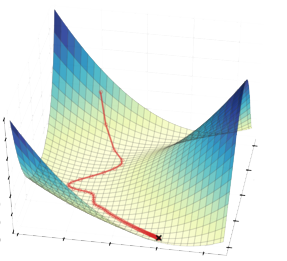
\includegraphics[width=.2\figwidth]{images/sgd.png}}
\label{fig:part2_math_sgd}
\caption{梯度下降}
\end{figure}

梯度是方向上升/下降最快的方向,它的幅值代表陡峭的程度。
所以,在最小值的地方,曲面轮廓几乎是平坦的,理论上最小值是梯度为0。
但事实上,我们又可能无法达到最小值,只能在最小值附近的平坦区域来回震荡。
当在这个区域震荡时,损失(Loss)值几乎是我们能达到的最小值了,并且不会有很大的变化,因此我们是在真实的最小值附近跳动。
通常,当损失值在预定的数字内没有改善的时候就会停止迭代,例如10次或者20次迭代。
当这种情况发生时,就说训练已经收敛了,或者说收敛已经完成了。

\subsection{BGD}
使用BGD(Batch Gradient Descent,批量梯度下降),在目标函数为凸函数时,虽然可以找到全局最优解,
但收敛速度慢,需要用到全部数据,因此内存消耗也大。因此,BGD不适用于大数据集。
其公式如下:

\noindent
$$\boldsymbol{W} \leftarrow \boldsymbol{W}-\eta \frac{\partial \boldsymbol{L}}{\partial \boldsymbol{W}}$$

\noindent
如公式所示,BGD的策略就是朝着当前所在位置的坡度最大的方向前进。
但它也有缺点,它在面对峡谷型函数时,效率会变得很低,呈现出震荡的姿态。

\subsection{SGD}
而SGD相当于BGD的升级版。SGD被称为随机梯度下降(Stochastic Gradient Desccent)。
正如它的名字所说,它首先通过mini-batch学习,
意思就是从训练数据中随机选择一部分数据(称为mini-batch),
将这些mini-batch作为对象,使用梯度法进行学习。
其代码如下所示:


\begin{lstlisting}[language=java]
	MultiLayerConfiguration conf = new NeuralNetConfiguration.Builder()
        .weightInit(WeightInit.XAVIER)
        .activation("relu")
        .optimizationAlgo(OptimizationAlgorithm.STOCHASTIC_GRADIENT_DESCENT)
        .updater(new Sgd(0.05))
        // ... other hyperparameters
        .list()
        .backprop(true)
        .build();
\end{lstlisting}


\subsection{Momentum}
Momentum也是一种常见的优化算法,也被称为SGD with Momentum。
恰如其名,它为了抑制SGD的震荡,在梯度下降过程中加入惯性。
简单来说,它就是在梯度越陡时,下降越快。较平缓时,下降较慢。
其公式如下:

$$\boldsymbol{v} \leftarrow \alpha \boldsymbol{v}-\eta \frac{\partial \boldsymbol{L}}{\partial \boldsymbol{W}}$$

$$\boldsymbol{W} \leftarrow \boldsymbol{W}+\boldsymbol{v}$$

\noindent
如上式所示,$\boldsymbol{W}$表示要更新的权重参数,$\frac{\partial L}{\partial \boldsymbol{W}}$
表示损失函数关于$\boldsymbol{W}$的梯度,$\eta$表示学习率。
而$\boldsymbol{v}$这一变量便是用来模拟惯性的。
其通过在SGD的基础上引入一阶动量,
这代表着现在下降方向不仅由当前点的梯度方向决定,而且由此前累积的下降方向决定。 


\begin{lstlisting}[language=java]
	MultiLayerConfiguration conf = new NeuralNetConfiguration.Builder()
        .weightInit(WeightInit.XAVIER)
        .activation("relu")
        .optimizationAlgo(OptimizationAlgorithm.STOCHASTIC_GRADIENT_DESCENT)
        .updater(new Nesterovs(0.05))
        // ... other hyperparameters
        .list()
        .backprop(true)
        .build();
\end{lstlisting}

\noindent
Momentum的更新路径就如同小球在碗中滚动一样。
与SGD相比,其大大缓解了震荡问题,原因就是它加入的一阶动量。
即使在某一方向“受力”很小,但因为其一直在同一方向受力,
所以它会朝着同一方向有一定的加速。
通俗地讲,就是它所加入的惯性,抵消了试图改变它的力。

\subsection{AdaGrad}
在梯度下降中,学习率的值很重要(记为$\eta$),
而在学习率的相关研究中,有一种被称为\textbf{学习率衰减}(learning rate decay)的方法,
随着机器学习的过程,使学习率逐渐减小。
它具体表现为,在一开始与其他方法类似,进行参数学习,
但在学习的过程中,当准确率越来越高时,便减少学习率。
其公式如下:
$$\boldsymbol{h} \leftarrow \boldsymbol{h}+\frac{\partial \boldsymbol{L}}{\partial \boldsymbol{W}} \odot \frac{\partial \boldsymbol{L}}{\partial \boldsymbol{W}}$$

$$\boldsymbol{W} \leftarrow \boldsymbol{W}-\eta \frac{1}{\sqrt{\boldsymbol{h}}} \frac{\partial \boldsymbol{L}}{\partial \boldsymbol{W}}$$

如公式所示,AdaGrad会为参数的每个元素适当地调整学习率,
与此同时进行参数的学习。AdaGrad的公式比起之前的,
新出现了一个变量$\boldsymbol{h}$,它代表着之前所有梯度值的平方和,
在更新参数时,通过乘以$\frac{1}{\sqrt{\boldsymbol{h}}}$,
AdaGrad便可以为每个元素调整适宜它的学习率。其代码如下所示:

\begin{lstlisting}[language=java]
	MultiLayerConfiguration conf = new NeuralNetConfiguration.Builder()
        .weightInit(WeightInit.XAVIER)
        .activation("relu")
        .optimizationAlgo(OptimizationAlgorithm.STOCHASTIC_GRADIENT_DESCENT)
        .updater(new AdaGrad(0.05))
        // ... other hyperparameters
        .list()
        .backprop(true)
        .build();
\end{lstlisting}
AdaGrad比起Momentum更好地抑制了SGD的震荡,函数的取值高效地向着最小值移动。
刚开始时,也许还会有些震荡,但越接近最小值,几乎是呈直线般向着目标前进。

\subsection{Adam}

\begin{lstlisting}[language=java]
	MultiLayerConfiguration conf = new NeuralNetConfiguration.Builder()
        .weightInit(WeightInit.XAVIER)
        .activation("relu")
        .optimizationAlgo(OptimizationAlgorithm.STOCHASTIC_GRADIENT_DESCENT)
        .updater(new Adam(0.05))
        // ... other hyperparameters
        .list()
        .backprop(true)
        .build();
\end{lstlisting}




\section{概率分布}

\section{损失函数}
在机器学习中,机器的学习需要某个指标来表示现在的状态,然后,以这个指标为基准,寻找最优权重参数。
而在机器学习中所用的指标便被称为\emph{损失函数}(loss function)。
对于损失函数,我们主要使用均方误差和交叉熵误差。

首先,我们介绍一种常用的函数,\emph{交叉熵误差}(cross entropy error)。
\begin{equation}
    E = - \sum _ { k } t _ { k } \log y _ { k }
    \label{part2_cross_entropy_error_1}
\end{equation}

在上式中,$y_{k}$代表着机器学习的输出,log表示以e为底数的自然对数($log_{e}$)。
$t_{k}$代表着正确解标签,仅当解标签为正确时,$t_{k}$的索引才为1。其余情况都为0。
因此,E所代表的实际为解标签为正确时所输出的自然对数。

%交叉熵误差的图像

如上图所示,当输出结果$y_{k}$越发趋向于1.0时,得到的E越发增大而趋向于0。
交叉熵误差通过E所表示的负值,来表明该权重参数与正确结果之间的偏差程度。

下面,我们用代码来实现交叉熵误差:
%代码
\begin{lstlisting}[language=Java,caption={交叉熵误差}]
\end{lstlisting}

%代码分析

%实际运行

\ \\
下面我们介绍另一种,在损失函数中最有名的\emph{均方误差}(mean squared error)。
它的公式如下所示:

\begin{equation}
    E = \frac { 1 } { 2 } \sum _ { k } \left( y _ { k } - t _ { k } \right) ^ { 2 }
    \label{part2_cross_entropy_error_2}
\end{equation}

在上式中k表示着数据处于哪一个维度,$t_{k}$表示着各维度的监督数据。通常情况下,
监督数据仅将正确解标签表示为1,而其他非正确解则表示为0。
而机器学习输出的结果$y_{k}$,则是会在各个维度都显示该维度是正确解标签的可能性。
均方误差通过计算机器学习的输出和正确解监督数据的各个元素之差的平方,再求总和。
从而得到该权重参数的输出结果与正确结果之间的偏差。

%代码
\begin{lstlisting}[language=Java,caption={均方误差}]
\end{lstlisting}

%代码分析

%实际运行

\section{拟合算法}

很多时候,我们希望通过一些样本来反应总体的特征,因此我们需要拟合曲线来判断总体的情况。 
假设有如下这些个样本,看起来各点分布趋于一条直线,因此我们希望通过一条直线来描述该样本所在总体的一些特征,对总体进行预测。一般的方法就是先假设一条直线,如L=ax+b,之后再根据前面这些样本,确定最优的a,b,所谓最优就是通过这些点计算出合适的a,b,使各个点对直线上垂直距离的平方和最小(最小二乘法)。具体的方法是通过迭代来计算的。













\chapter{微积分}
\label{chap:calculus}
微积分(Calcuus)是数学的一个基础学科,包括极限、微分学、积分学及其应用。
与机器学习相关的微积分问题有:极值问题、偏导数和梯度。
在机器学习中,定义的所谓模型就是一个包含参数和特征的函数。
定义如下:
$$h_{\theta}(x)=\theta_0+\theta_1x_1+\theta_2x_2+\theta_3x_3+\dots+\theta_nx_n$$
其中,$\theta_i$称为参数,而$x_i$称为特征,$h_{\theta}$是预测模型。
训练模型之前,都会采集很多组样本数据$(x_1, x_2, \dots, x_n)$,
$x_i$就是预设的特征。
模型的准确性,取决于特征的完备性和数据的充分性。
取什么样的特征(采集什么样的数据)有时候也很难确定,过少的或过多的特征,都影响模型的准确性。

\begin{figure}[!htb]
	\centerline{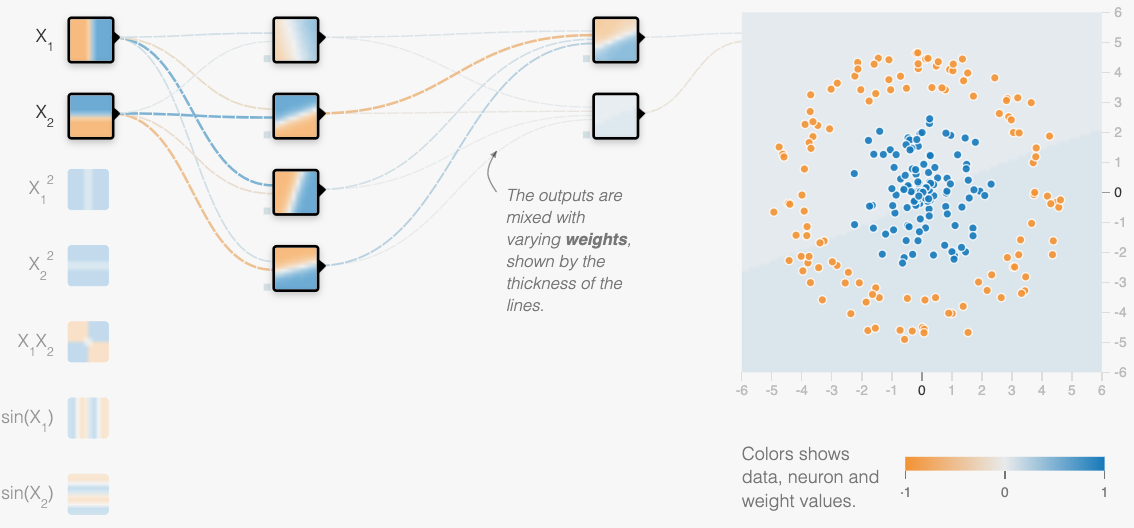
\includegraphics[width=.50\figwidth]{images/x1x2relu.png}}
	\caption{线性特征分类}
	\label{fig:part2_math_x1x2relu}
\end{figure}

极端情况下,已有的样本数据少于特征的维度(相当于未知数多于方程个数),需要引入$\lambda$正则项。
通过\emph{岭回归}(Ridge Regression)得出最优的$\lambda$和$\theta$,下一章线性代数部分会详细说明。

如果特征值$(x_1, x_2, \dots, x_n)$向量线性相关,就有必要减少特征的维度。
很显然,特征空间的维度降低可以极大地简化模型。
采集的样本数据通常都有一些噪点,要引入正则化降低它们对训练结果的影响,防止\emph{过拟合}的出现。
注意,\emph{欠拟合}是指模型包含的特征维度低于现实情况,也无法训练出有效的结果。

由\figref{fig:part2_math_x1x2relu}可知,两个线性特征x1和x2通过线性组合只能训练出多边形特征的模型。
加入特征x3并定义为$x_1^2$,特征x4定义为$x_2^2$,改进后的模型分类预测更符合预期。
实际上,需要哪些特征也并不是那么很明显。首先是我们能获取到哪些数据,主观判断是否相关。
譬如,你可以拿到的数据:(年龄,性别,身高,体重,籍贯),想用于预测某人的籍贯。
$$f(\text{年龄,性别,身高,体重}) -> \text{籍贯}$$

在定义模型之后,通常使用最小二乘法定义\emph{损失函数}(代价函数,Cost Function)。
然后把准备好的大量样本喂给模型,进行迭代训练使其学习出最优的$\vec{\theta}$,
使得代价函数的值尽量小。

$$J(\theta_0, \theta_1, \dots, \theta_n) = \frac{1}{2m}\sum_{i=1}^m(y^i-h_\theta(x^i))^2$$

在机器学习中,使用激活函数对结果进行逻辑分类:
Sigmoid函数,
Tanh函数,
ReLu函数。
它们的主要区别是什么?请同学们仔细观察函数图形之间的共性和区别。

\begin{figure}[!htbp]
\centering
\begin{minipage}{0.33\textwidth}
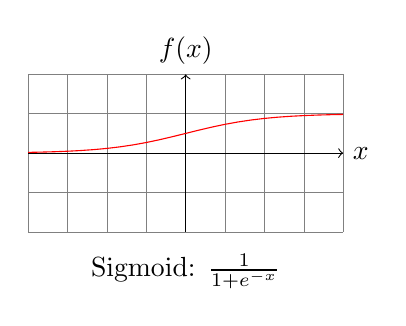
\begin{tikzpicture}[scale=0.5]
  \draw[very thin,color=gray] (-4,-2) grid (4,2);
  \draw[->] (-4,0) -- (4,0) node[right] {$x$};
  \draw[->] (0,-2) -- (0,2) node[above] {$f(x)$};
	\draw[color=red, domain=-4:4] plot (\x,{1/(1+e^-\x)});
	\node at (0, -3) {Sigmoid: $\frac{1}{1+e^{-x}}$};
\end{tikzpicture}
\end{minipage}%
\begin{minipage}{0.33\textwidth}
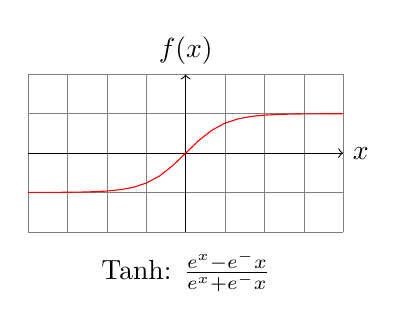
\begin{tikzpicture}[scale=0.5]
  \draw[very thin,color=gray] (-4,-2) grid (4,2);
  \draw[->] (-4,0) -- (4,0) node[right] {$x$};
  \draw[->] (0,-2) -- (0,2) node[above] {$f(x)$};
	\draw[color=red, domain=-4:4] plot (\x,{(e^\x-e^-\x)/(e^\x+e^-\x)});
	\node at (0, -3) {Tanh: $\frac{e^x-e^-x}{e^x+e^-x}$};
\end{tikzpicture}
\end{minipage}%
\begin{minipage}{0.33\textwidth}
	\vspace{0.55cm}
	\begin{tikzpicture}[scale=0.5]
		\draw[very thin,color=gray] (-4,-2) grid (4,2);
		\draw[->] (-4,0) -- (4,0) node[right] {$x$};
		\draw[->] (0,-2) -- (0,2) node[above] {$f(x)$};
		\draw[color=red, domain=-4:0] plot (\x,0);
		\draw[color=red, domain=0:2] plot (\x,\x);
	\node at (0, -3.2) {ReLu: 
			$\begin{cases} 
				x&\text{x>=0}\\0&\text{x<0}
			\end{cases}$};
	\end{tikzpicture}
\end{minipage}%
\end{figure}
引入激活函数不仅用于逻辑分类,关键是还引入了非线性因素。
Sigmoid函数的输出在(0,1)之间,单调连续,并且容易求导。
但它一旦输入落入饱和区,一阶导数就会接近于0,容易产生梯度消失;
Tanh函数也是传统神经网络中常用的激活函数,与Sigmoid一样存在饱和问题。
不过它的输出以0为中心,Tanh函数看上去是放大的Sigmoid函数。

ReLu是目前用的最多也是最受欢迎的激活函数,可加速SGD(梯度下降算法) 的收敛。
但ReLu随着训练的进行,部分输入也会落到硬饱和区。
除了ReLu,还许多ReLu衍生的激活函数,比如:Leaky ReLu、ReLU6、SReLu、PReLu、RReLu、CReLu。


\section{偏导数与梯度}
在微分中,导数表示函数的变化率,也是变化率最大的方向。
梯度是全部偏导数构成的向量,一般将函数$f$的梯度记为$\Delta f$。
根据方向导数的知识,可知梯度的方向即为函数值增长最快的方向。

$$ grad f(x_0, x_1,\cdots, x_n) = (
		\frac{\delta f}{\delta x_0},
		\frac{\delta f}{\delta x_1},
		\cdots,
		\frac{\delta f}{\delta x_n}
) $$

\noindent
函数在某一点的梯度,是一个向量,与最大方向导数的方向一致,
而它的模就是方向导数的最大值。
既然,沿梯度方向具有最大的变化率,所以沿着负梯度方向去减小函数值,
才能最快达到优化目标。

\begin{figure}[!h]
\centering
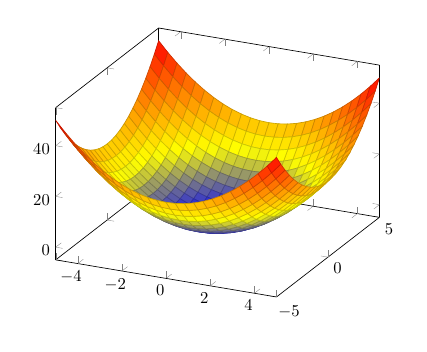
\begin{tikzpicture}[scale=0.6]
	\begin{axis}
	\addplot3[surf]                % 绘制三维图
	 {x^2+y^2};                    % 输入二元显式函数
	\end{axis}
\end{tikzpicture}
\hspace{0.1cm}
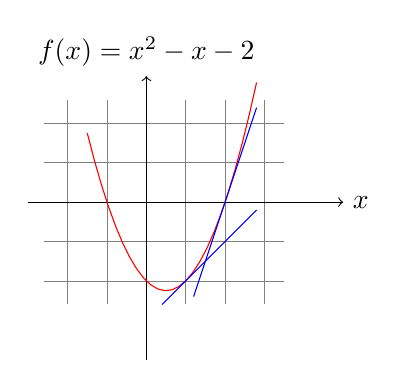
\begin{tikzpicture}[scale=0.5]
  \draw[very thin,color=gray] (-2.6,-2.6) grid (3.5,2.6);
  \draw[->] (-3,0) -- (5,0) node[right] {$x$};
  \draw[->] (0,-4) -- (0,3.2) node[above] {$f(x)=x^2-x-2$};
	\draw[color=red, domain=-1.5:2.8] plot (\x,{\x*\x-\x-2});
	\draw[color=blue, domain=1.2:2.8] plot (\x,{3*\x-6});
	\draw[color=blue, domain=0.4:2.8] plot (\x,{\x-3.0});
\end{tikzpicture}
\end{figure}

\noindent
梯度下降就像是你低头只看脚下的下山过程,若想最快到达山底,
最好每一步都找最陡峭的方向走,这就是梯度的负方向。由于视野的局限性,
使用\emph{梯度下降}也有可能落入局部最小值。

\ \\
\noindent \emph{例子}
	函数 $f(x)=x^2-x-2$, 梯度:$f'(x) = 2x-1$
\begin{lstlisting}[numbers=none]
假设α=0.2可以这样推算: 设起点为(4,0)

1次:参数x=4, 4-0.2*(2*4-1)=2.6
2次:参数x=2.6, 2.6-0.2*(2*2.6-1)= 1.76 
3次:参数x=1.76, 1.76-0.2*(2*1.76-1)=1.256 
4次:参数x=1.256, 1.256-0.2*(2*1.256-1)=0.9536 
5次:参数x=0.9536, 0.9536-0.2*(2*0.9536-1)=0.77216 
......
After 13 steps: x = 0.502743, f(x)= -2.249992. 
After 14 steps: x = 0.501646, f(x)= -2.249997. 
After 15 steps: x = 0.500987, f(x)= -2.249999. 
After 16 steps: x = 0.500592, f(x)= -2.250000. 
After 17 steps: x = 0.500355, f(x)= -2.250000. 
After 18 steps: x = 0.500213, f(x)= -2.250000.
\end{lstlisting}

\section{线性拟合}
样本的散点图有助于发现关键特征,建立正确的模型。
如下图,可直观地识别出线性关系,尽管有干扰数据。
\begin{figure}[!h]
	\begin{center}
	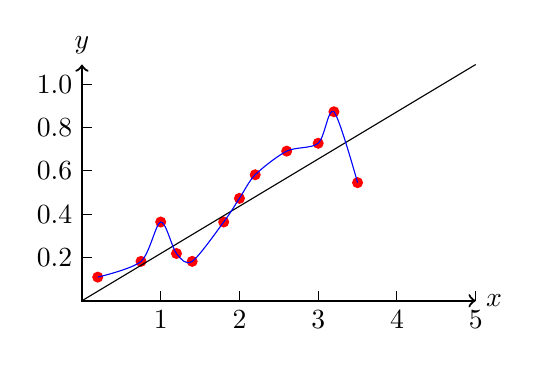
\begin{tikzpicture}
			\pgfmathsetmacro{\ticker}{0.125}
			\draw [<->,thick] (0,3) node (yaxis) [above] {$y$}
							|- (5,0) node (xaxis) [right] {$x$};
			\foreach \i/\texti  in {1,2,3,4,5} {
			\draw (1*\i,0) --(1*\i,\ticker) node[label=below:\texti]{};
			}
			\foreach \j/\textj  in {0.2,0.4,0.6,0.8,1.0} {
			\draw (0,2.75*\j) --(\ticker,2.75*\j) node[label=left:\textj]{};
			}
			\
			\fill[red] (0.2,0.3) circle (2pt);
			\fill[red] (0.75,0.5) circle (2pt);
			\fill[red] (1,1) circle (2pt);
			\fill[red] (1.2,0.6) circle (2pt);
			\fill[red] (1.4,0.5) circle (2pt);
			\fill[red] (1.8,1) circle (2pt);
			\fill[red] (2.0,1.3) circle (2pt);
			\fill[red] (2.2,1.6) circle (2pt);
			\fill[red] (2.6,1.9) circle (2pt);
			\fill[red] (3,2.0) circle (2pt);
			\fill[red] (3.2,2.4) circle (2pt);
			\fill[red] (3.5,1.5) circle (2pt);
			\draw (0,0) -- (5,3) node [] {};
			\draw[blue] plot[smooth] coordinates{
				(0.2,0.3) (0.75,0.5) (1,1) (1.2,0.6) (1.4,0.5)
				(1.8, 1)  (2.0,1.3) (2.2, 1.6) (2.6, 1.9) 
				(3, 2.0) (3.2,2.4) (3.5, 1.5) };
			\end{tikzpicture}
			\caption{线性拟合}
	\end{center}
\end{figure}

拟合指的是你逼近目标函数的远近程度。
\emph{欠拟合},是指模型复杂度过低,不能很好的拟合所有的数据,训练误差大,在训练和预测时表现都不好。
欠拟合很容易被发现,在训练的时候就表现很差。
\emph{过拟合},是指模型复杂度很高,但训练数据很少,导致训练误差小,测试误差也大。
过拟合,过度地学习训练数据中的细节和噪音,以至于模型在新的数据上表现很差,泛化性能变差。
\footnote{欠拟合(underfitting),或者叫作叫做高偏差(bias),过拟合(overfitting),也叫高方差(variance)}

\begin{figure}[!htb]
	\centerline{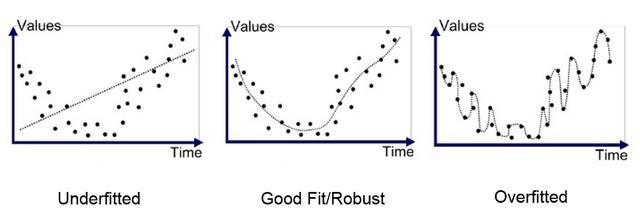
\includegraphics[width=.50\figwidth]{images/overfit_underfit.png}}
	\caption{拟合情况分类}
	\label{fig:part2_math_overfit_underfit}
\end{figure}

\subsection{最小二乘法}
最小二乘法是勒让德( A. M. Legendre)于1805年在其著作《计算慧星轨道的新方法》中提出的。
它的主要思想就是求解未知参数,使得理论值与观测值之差(即误差,或者说残差)的平方和达到最小。

$$E = \sum_{i=1}^n(y_i-\hat{y})\footnote{$y_i$是样本数据,$\hat{y}$是理论值}$$

\section{优化问题}
拉格朗日乘子法(Lagrange Multiplier),用于求解带等式约束的极值问题,而KKT(Karush Kuhn Tucker)条件是拉格朗日乘子法的推广。
在有等式约束时使用拉格朗日乘子法,在有不等约束时使用KKT条件。

\subsection{拉格朗日乘子}
拉格朗日乘子法是一种寻找多元函数在其变量受到一个或多个条件的约束时的极值的方法。
设目标函数为$f(x)$,约束条件为$h_k(x)$,其中s.t. 表示subject to ,“受限于”的意思,$l$表示有$l$个约束条件。
定义如下:

$$L(x,\lambda)=f(x)+\lambda h_k(x)$$
\[
min \enskip f(x) \quad \vert \quad s.t. \enskip h_k(x) = 0 \quad k=1,2,\dots,l
\]

\begin{enumerate} \setlength{\parsep}{0pt} \setlength{\parskip}{0pt}
	\item 构造拉格朗日函数 
	\item 解偏导方程 
	\item 代入上述函数 
\end{enumerate}

由拉格朗日乘子法的定义可知,它是一种寻找极值的方法,因此该方法并不能保证极值点是最低点或者最高点。
\begin{figure}[!htb] \centering 
	\begin{tikzpicture}
		\node at (0,0) {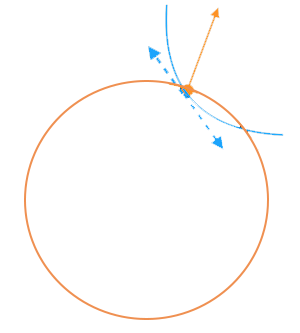
\includegraphics[width=3.5cm]{images/orange-gradient.png}};
		\node at (4,0) {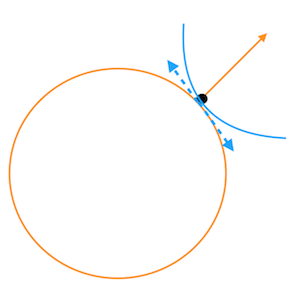
\includegraphics[width=4cm]{images/black-gradient.png}};
		\node at (8,0) {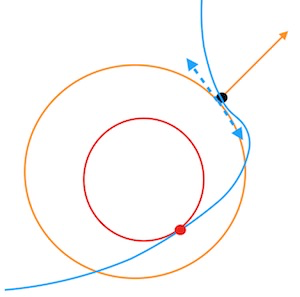
\includegraphics[width=4cm]{images/multiple-solution.png}};
		\node at (0,1.5) {图1};
		\node at (4,1.5) {图2};
		\node at (8,1.5) {图3};
	\end{tikzpicture}
	\caption{拉格朗日算子法}
\end{figure}

这里不加任何推导,很明显相切的时候才能到最低点。
橙线的梯度(上图1橙色箭头)和蓝线的切线(蓝色虚线)不是垂直关系。
蓝线的两个切线方向,分布往函数高处走(与梯度的夹角小于 90 度),和往函数低处走(与梯度的夹角大于 90 度)。
因此,两条曲线相交时,肯定不在最低点或最高点的位置。

如果两条曲线相切(上图2),那么蓝线的切线和橙线的梯度是在切点这个位置垂直。
这时,蓝线的切线方向指向橙线的等高线方向。
图3中相切的点有两个,而红点的明显比黑点小。
要判断找到的点是极低点还是极高点,需要将切点代入原函数再进行判断。
在实际求解时,令各偏导为0就能满是相切的条件。

\subsection{KKT条件}
在优化理论中,KKT条件是非线性规划(Nonlinear Programming)最优解的必要条件。
KKT条件将拉格朗日算子法中的等式约束优化问题推广至不等式约束。
将上一节中的约束等式$h_k(x)=0$推广为$g_i(x) \le 0$,优化问题如下:

\[
	min \enskip f(x) \quad \vert \quad s.t. g(x) \le 0
\]

约束不等式$g(x) \le 0$称为Primal Feasibility,
定义可行域为(Feasible Region)$K=\{x\in\mathbb{R}n∣g(x) \le 0\}$。
设$x^\star$为满足约束条件的最优解,可分为内部解、边界解两种情况。
内部解的时候,$g(x)$不起作用,退化为无约束问题。
边界解的时候,取不等式的边界,约束转换为$g(x)=0$,转化为Lagrange算子法。

\begin{enumerate}
	\item $g(x^\star) \le 0$,最佳解位于K的内部,此时约束条件是无效的;
	\item $g(x^\star)=0$,最佳解落在K的边界,此时约束条件是有效的。
\end{enumerate}

\begin{figure}[!htb] \centering 
	\begin{tikzpicture}
		\node at (0,0.3) {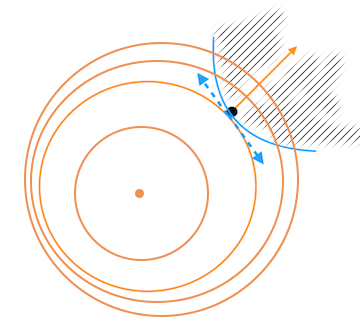
\includegraphics[width=4cm]{images/kkt-region.png}};
		\node at (4,0) {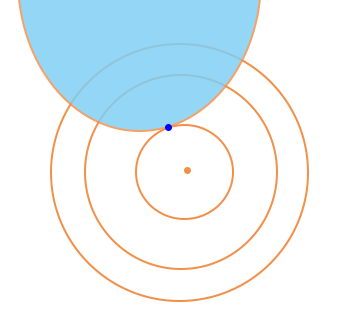
\includegraphics[width=4cm]{images/kkt-cond.png}};
		\node at (8,0) {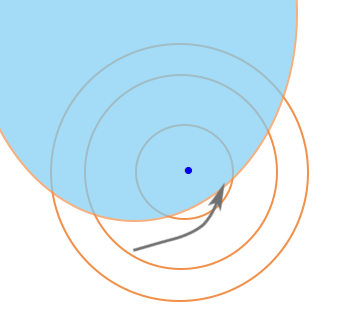
\includegraphics[width=4cm]{images/kkt-cond-2.png}};
		\node at (0,1.5) {图1};
		\node at (4,1.5) {图2};
		\node at (8,1.5) {图3};
		\node at (3.6,0.4) {$x^*$};
		\node at (8,0) {$x^*$};
		\node at (3,0.8) {$g_i(x)=0$};
		\node at (7,-1.3) {$g_i(x)=0$};
	\end{tikzpicture}
	\caption{KKT}
\end{figure}

KKT-图1中,把Lagrange条件变成一个区域,该图的切点处仍旧是最优解。
KKT-图2中,在边界处$g(x)=0$等价于Lagrange算子法。
KKT-图3中,最佳解位于K的内部,约束条件无效。
KKT是SVM(support vector machine)支持向量机的重要理论基础。

\subsection{凸优化}
凸优化在数学规划领域具有非常重要的地位。
若能把一个实际问题表述为凸优化问题,基本上意味着该问题已经得到解决,这是非凸的优化问题所不具有的性质。
机器学习中有很多优化问题都要通过凸优化来求解,即便是在非凸优化中,凸优化同样起着重要的作用。
实际上,很多非凸优化问题,可以转化为凸优化问题来解决。

$$
f_i(\alpha x + \beta y) \le \alpha f_i(x) + \beta f_i(y),
\quad
\text{其中} \alpha + \beta = 1, \alpha \ge 0, \beta \ge 0
$$

\begin{figure}[!htb]
	\centerline{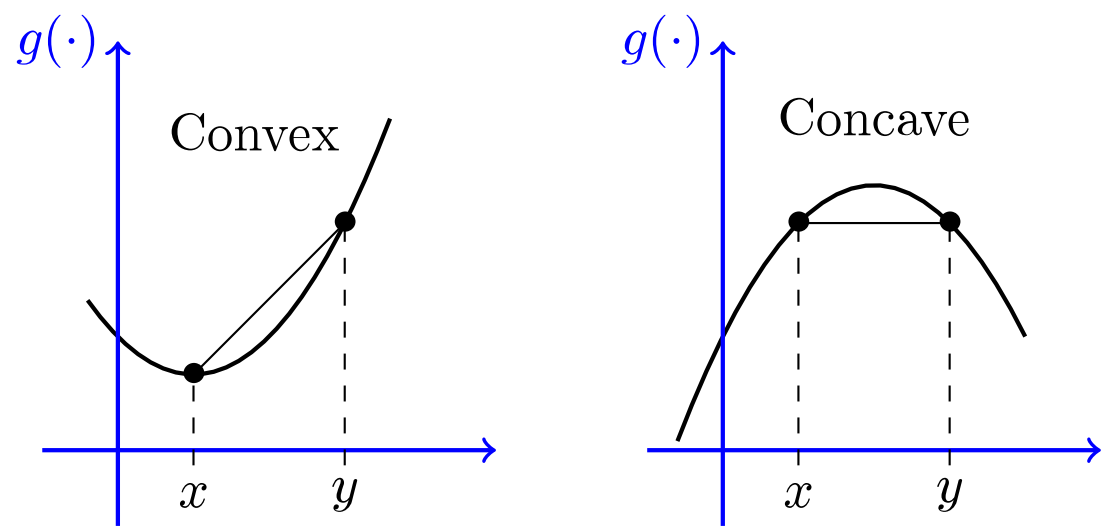
\includegraphics[width=.30\figwidth]{images/convex-concave.png}}
	\caption{凸函数和凹函数}
	\label{fig:part2_math_convex_concave}
\end{figure}

如\figref{fig:part2_math_convex_concave}所示,
凸函数的几何意义为任意两点连线上的取值大于该点在函数上的取值,
而凹函数正好相反。很显然,凸函数总是在其任意一点的切线的上方。
通常使用函数的二阶导来判断一个函数是否为一个凸函数。

$$
\bigtriangledown_x^2f(x) \ge 0
$$

\begin{figure}[!htb]
	\centerline{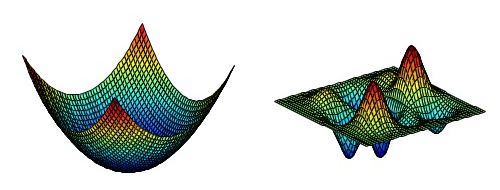
\includegraphics[width=.35\figwidth]{images/concave-to-convex.png}}
	\caption{凹函数转化为多个凸函数优化问题}
	\label{fig:part2_math_concave_to_convex}
\end{figure}

凸优化相对简单,具有良好的几何性质,比如分离平面和支撑平面。
通常凸问题的局部最优解也是全局的最优解,Lagrange对偶是凸优化理论中最重要的工具。
往往只要把某一问题抽象为凸问题,就可近似认为这个问题已经解决了。

SVM本身就是把一个分类问题抽象为凸优化问题,利用凸优化的各种工具(如Lagrange对偶)求解和解释。
深度学习中关键的算法是反向传播(Back Propagation),本质就是凸优化算法中的梯度下降算法。
总的来说,凸优化在工程领域的应用中有着无可撼动的地位。

实际上,生活中几乎所有问题的本质都是非凸的。
如\figref{fig:part2_math_concave_to_convex}所示,
很多非凸问题可以转化成多个凸优化问题,加速问题的求解。

\section{损失函数}
在机器学习中,机器的学习需要某个指标来表示现在的状态,然后,以这个指标为基准,寻找最优权重参数。
机器学习利用已知样本,推演隐藏在背后的真实曲线。这里假设该某曲线为
$h_{\theta}=\theta_0+\theta_1x+\theta_2x^2+\theta_3x^3+\theta_4x^4$ ,
通过样本求解$\theta_i$($i=0\cdots4$)。
不过,这个假设(Hypothesis)很有可能不是最好的。
实际上,我们获得的训练数据总是有误差,不能完全拟合这些数据点,否则就会导致\emph{过拟合}(overfit)的问题。

评价训练过程是否有效,可使用方差衡量源数据和期望值相差的偏离程度。
若是逐渐减小,就是一个有效的训练过程。
这个方差也是一个函数,称为\emph{损失函数}(loss function)\footnote{也称为代价函数(Cost Function)},
用于计算预测值f(x)与真实值y的不一致程度。
它是一个非负的实值函数,通常使用L(Y, f(x))来表示。损失函数值越小,拟合效果就越好。
当样本个数为n时,此时的损失函数变为:
$$
L(Y, f(x)) = \frac{1}{N}\sum\limits_{N}(Y-f(x))^2
$$
$$\text{除2是为了方便求导}$$
$Y-f(X)$表示的是残差,整个式子表示的是残差的平方和,而我们的目的就是最小化残差的平方和。
在实际应用中,通常使用\emph{均方误差}(mean squared error)作为衡量指标,如下:
$$
E=\frac{1}{2} \sum_{k}\left(y_{k}-t_{k}\right)^{2}
$$
在上式中k表示着数据处于哪一个维度,$t_{k}$表示着各维度的监督数据。通常情况下,
监督数据仅将正确解标签表示为1,而其他非正确解则表示为0。
而机器学习输出的结果$y_{k}$,则是会在各个维度都显示该维度是正确解标签的可能性。
均方误差通过计算机器学习的输出和正确解监督数据的各个元素之差的平方,再求总和。
从而得到该权重参数的输出结果与正确结果之间的偏差。

我们现在再介绍另一种常用函数,\emph{交叉熵误差}(cross entropy error)。
其公式如下:
$$
E=-\sum_{k} t_{k} \log y_{k}
$$

在上式中,$y_{k}$代表着机器学习的输出,log表示以e为底数的自然对数($log_{e}$)。
$t_{k}$代表着正确解标签,仅当解标签为正确时,$t_{k}$的索引才为1。其余情况都为0。
因此,E所代表的实际为解标签为正确时所输出的自然对数。


线性回归是确定两个或两个以上变量间关系的一种常见统计分析方法,被广泛用于回归分析。
只有一个自变量的情况称为简单回归,多于一个自变量的情况叫做多元回归。
故可分为一元线性回归分析方程和多元线性回归分析方程。
给定一个随机样本($Y_i, X_i1, \cdots, X_ip$),线性回归模型表示为以下的形式:
$$Y_i = \beta_0+\beta_1X_{i1}+\beta_2X_{i2}+\cdots+\beta_pX_{ip}+\epsilon_i$$
$$i=1,\cdots,n.$$

使用最小二乘法(Least Square Method)需要做矩阵的逆运算,下一章我们再介绍。
而\emph{梯度下降}法起点和学习率都非常重要,顺着梯度$\Delta$下降最快的方向迭代调整。
若干次迭代之后就会落入局部最小点附近,有可能来回震荡无法达到极值点。
所以,调整学习率就非常关键,因此到极值点附近的时候收敛速度也会变慢。




\subsection{反向传播(Back Propgation)}
前述几节,我们利用偏导获得梯度,然后逐步调节参数,朝着误差越来越小的方向迭代。
这还算不上神经元,实际比这还要复杂一些,通常还有一个激活函数(Activation Function),
只有对神经元的刺激足够强才会前向传递。
典型的深度神经网络,至少包含:输入层、隐藏层、输出层。

\begin{figure}[!htb] \centering 
	\begin{tikzpicture}
		\node at (0,0) {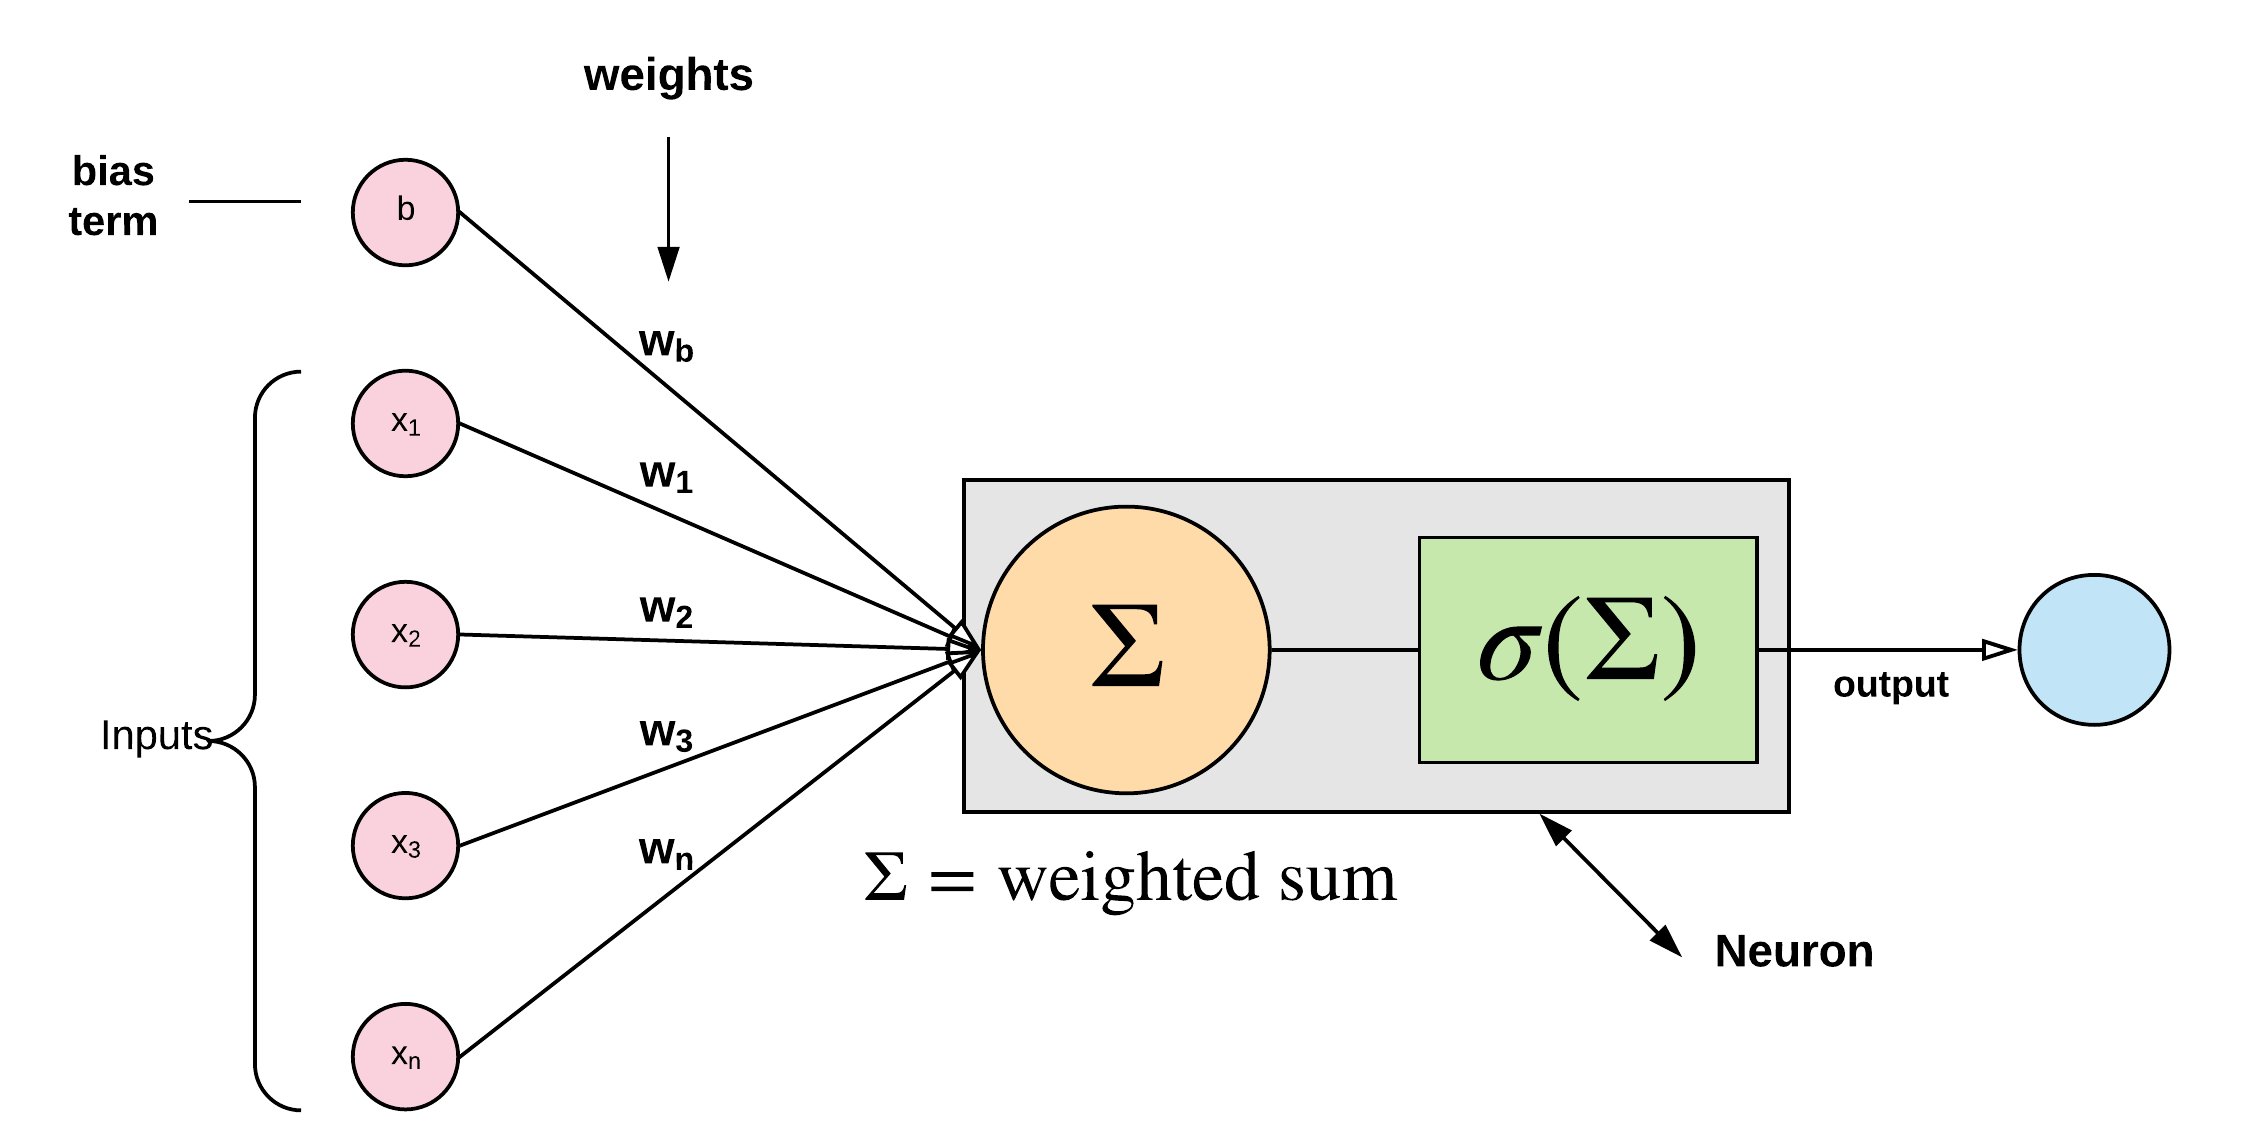
\includegraphics[width=\textwidth]{images/activation-function.png}};
		\node at (1,1) {$\sigma = \text{激活函数}$};
	\end{tikzpicture}
	\caption{神经网络}
	\label{fig:part2_math_neural_node}
\end{figure}

缺少激活函数的线性模型,甚至都无法解决异或问题。
如果选用Linear函数$g(x)=x$作为激活函数就无法划分下图的区域,很显然隐藏层的混入也非常关键。
通过隐藏层引入了更多线段,以便合成一个封闭的多边形,恰好能对数据分类。
激活函数可以在隐藏层引入更多特征,产生非线性结果以解决线性不可分问题。

\begin{figure}[!htb] \centering 
	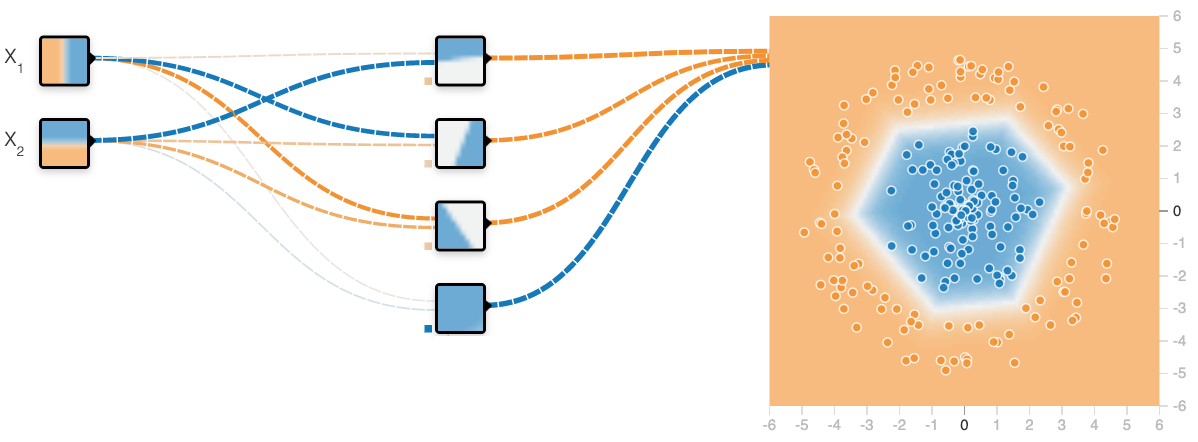
\includegraphics[width=\textwidth]{images/reLu-x1-x2.png}
	\caption{使用激活函数,合成多边形区域}
	\label{fig:part2_math_neural_linear}
\end{figure}


BP神经网络是一种多层的前馈神经网络,分为两个阶段:前向传播和反向传播。
前向传播从输入层经过隐含层,最后到达输出层。
而反向传播从输出层到隐含层,最后到输入层,
逐步调节隐藏层(Hidden Layer)到输出层的权重和偏置(bias),输入层到隐含层的权重和偏置。
经由反向传播,把误差反馈给神经网络用于调节参数。此处不作严格证明,

假设有一个两层深的网络(1个隐藏层),并且每一层只有一个神经元,
$\sigma$为\emph{sigmoid}函数。
相应的数学模型如下:
\begin{figure}[!htb] \centering 
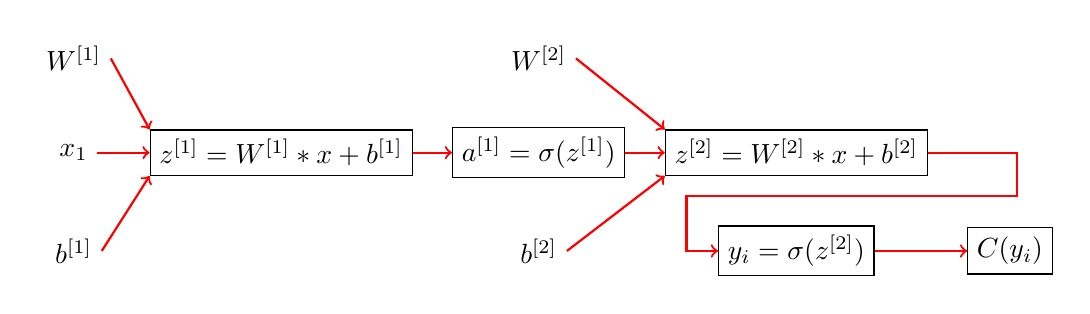
\begin{tikzpicture}
	\matrix [column sep={5mm,between borders}, row sep = 6mm]
	{
		\node (w1) {$W^{[1]}$}; 
			& \node{};
			& \node(w2) {$W^{[2]}$};
			& \node{};
			& \node{}; \\
		
		\node (x1) {$x_1$}; 
			& \node[draw] (n1) {$z^{[1]}=W^{[1]}*x + b^{[1]}$}; 
			& \node[draw] (o1) {$a^{[1]} = \sigma(z^{[1]})$};
			& \node[draw] (n2) {$z^{[2]}=W^{[2]}*x + b^{[2]}$}; 
			& \node{};\\
		
		\node (b1) {$b^{[1]}$}; 
			& \node{}; 
			& \node(b2) {$b^{[2]}$};
			& \node[draw] (o2) {$y_i = \sigma(z^{[2]})$};
			& \node[draw] (C) {$C(y_i)$}; \\
	};
	\draw [->,red,thick] (w1.east) -- (n1.north west) node {};
	\draw [->,red,thick] (x1.east) -- (n1.west) node {};
	\draw [->,red,thick] (b1.east) -- (n1.south west) node {};
	\draw [->,red,thick] (n1.east) -- (o1.west) node {};
	\draw [->,red,thick] (o1.east) -- (n2.west) node {};
	\draw [->,red,thick] (w2.east) -- (n2.north west) node {};
	\draw [->,red,thick] (b2.east) -- (n2.south west) node {};
	\draw [->,red,thick] (n2.east) -| (6,-0.5) -| (1.8, -0.5) |- (o2.west) node {};
	\draw [->,red,thick] (o2.east) -- (C.west) node {};
\end{tikzpicture}
\end{figure}

\noindent
从输入到输出,函数都是平滑的可求偏导的,由误差估计$C(\hat{y})$使用梯度下降法,反向调节参数。
其中, $a^{[i]}$作为下一个神经元的输入,也就是$x_i$。
$$
\frac{\partial{C}}{\partial{b_1}} 
= 
	\frac{\partial{C}}{\partial{y_i}} \cdot
	\frac{\partial{y_i}}{\partial{z_2}} \cdot
	\frac{\partial{z_2}}{\partial{a_1}} \cdot
	\frac{\partial{a_1}}{\partial{z_1}} \cdot
	\frac{\partial{z_1}}{\partial{b_1}}
= 
	\frac{\partial{C}}{\partial{y_i}} \cdot
		\sigma^{'}(z_2) \cdot W_2 \cdot \sigma^{'}(z_1)
$$


如\figref{fig:part2_math_neural_node},
神经网络的输入层就是我们要分类的样本特征,
而隐藏层和输出层每个节点都代表了一个sigmoid单元。
计算的时候,通常把b转化为$x_0$和$w_0$,可把sigmoid单元简化为$net=\sum_{i=0}^nW_ix_i$。
求各输入的和用sigmoid函数得到输出$out=\sigma(net)=\frac{1}{1+e^{-net}}$,
这便是一个单元的计算过程。

整个网络便是前一层作为输入与后一层的每各单元连接,计算出各单元的输出后,再把这一层做为输入传递到后一层。
算法本身并不复杂,隐含在其中的数学推理比较晦涩,包含的过程主要是梯度下降和函数迭代。


\chapter{概率与分布}
\label{chap:regression}

日常生活中,我们差不多一直在做各种判断,这样或者那样。俗话说,选择大于努力。如果你的认知或者价值观是错误的,将不会得出正确的结果。
这种价值观的偏离,需要“\emph{误差分析}”保证在正确的轨道上。然而,误差很难线性(任意曲线)吻合的,这取决于个人的生活经验,

\begin{figure}[!htb]
\centerline{
\includegraphics[width=.1\figwidth]{images/4or9.png}}
\centerline{手写数字:4还是9?}
\end{figure}

如上图,手写数字很不容易判断,只能根据大多数人的情况猜测。
如果,你能拿到该人之前的手稿了解一下,就能有99.999\%概率做出正确判断。

有很多情形,我们也很难正确判断,只需要\emph{人工智能}输出TOPN可能性。
譬如,仅根据病人是否发烧、咳嗽难以确诊是否肺炎。进一步,借助沟通和血液化验,才更加确诊病人的实际病症。
这也只能说是99.99\%的准确率,即使是非常有经验的医生也有误诊的概率,只是非常小而已。

\emph{人工智能}研究的多是不确定性问题,需要你掌握概率和统计学的基础知识。
现实生活中,很多不确定事件都服从某种分布,譬如公交地铁站客流量服从泊松分布,而
1小时内到银行办理业务的客户数都也服从泊松分布(Poisson distribution)。
泊松分布具有以下特点:
\begin{itemize}
\item[1.] 无限分隔为若干小时间段,在这接近于零的小时间段里,发生1次的概率与时间段的长度成正比。
\item[2.] 在每一个极小时间段内,该事件发生两次及以上的概率恒等于零。
\item[3.] 在不同的小时间段里,发生与否相互独立。
\end{itemize}
\vspace{0.3cm}
\begin{equation*}
P\left( x \right) = \frac{{e^{ - \lambda } \lambda ^x }}{{x!}}
\end{equation*}

\noindent
泊松分布服从上述公式,很显然它所有事件的概率和等于1。
\begin{equation*}
\frac{{e^{-\lambda}\lambda^x }}{{x!}}
=e^{-\lambda }\left( \frac{{ \lambda ^x }}{{x!}}\right)
=e^{-\lambda } * e^\lambda
=1
\end{equation*}

\begin{lstlisting}[language=java]
在医疗质量上,美国误诊率是30-40%之间,因医疗差错而死亡的人,仅次于心血管疾病与肿瘤。
个别疾病的误诊率高得使你不敢想象,达到70%以上。
我国的误诊率尚没有公认的数据,但与美国相比只会高不会低。
\end{lstlisting}

\section{全概率公式}

全概率公式是概率论中重要的公式。他的意义在于直接计算$P(A)$比较困难时,可以将事件$A$分解为几个
小事件$B_i$,通过计算这些小事件的概率和,从而达到简化问题的效果。


全概率公式可以用如下的公式表示:
\begin{equation}
    P(A)=\sum_{i=1}^{\infty} P\left(B_{i}\right) P\left(A | B_{i}\right)
\end{equation}

\noindent
其中,事件$B_1,B_2,B_3,...,B_n$需要满足完备事件组,
即两两之间不能有交集,它们的和为全集,且概率大于零。
这样,事件$A$就被分解成了小事件$AB_1,AB_2,AB_3,...,AB_n$,由概率的加法公式即可得出
事件$A$的概率。


与全概率公式相反,贝叶斯公式是基于$P(A)$已知的前提下,寻找事件发生的原因$P(B_i|A)$。
贝叶斯公式可以用以下公式表示:
\begin{equation*}
    P\left(B_{t} | A\right)=\frac{P\left(B_{i}\right) P\left(A | B_{i}\right)}{\sum_{j=1}^{n} P\left(B_{j}\right) P\left(A | B_{j}\right)}
\end{equation*}

\noindent
其中事件$B_1,B_2,B_3,...,B_n$须满足完备事件组。

\section{最大似然}

最大似然估计是一种统计方法,用来求一个样本集的相关概率密度函数的参数。通俗地来讲,
就是通过已知的样本结果,反推最有可能出现这样结果的参数值。

例如,假设一个口袋中同时存在黑球和白球,我们从中随机抽取十个球,得到了8个黑球和2个白球。
在求解最有可能的黑白球比例时,我们就会采用最大似然法:假设从中抽到黑球的概率为$p$,
那么得到8次黑球2次白球的概率为:

\begin{equation*}
  P(A)=p^{8}*(1-p)^2
\end{equation*}

\noindent
在这个公式中,使$P(A)$达到最大的$p$值即为我们要求的结果。这就是最大似然问题的基本过程。


\section{期望与方差}

期望也称数学期望,在概率论与数理统计中指的是一个离散型随机变量在实验中每次可能的结果乘上
各自的概率的总和。在机器学习中,期望值是衡量一组数据离散程度的重要度量。

期望值的计算用以下公式表达$\mathrm{E}[X]=\sum_{i} p_{i} x_{i}$,其中$\mathrm{E}[X]$代表
期望值,$x_{i}$和$p_{i}$分别代表每次随机变量实验的可能结果与出现的概率。

与期望值类似,方差是概率论中衡量随机变量离散程度的度量。它具体指每个样本值与全体样本值平均数
之差的平方值的平均数。一般情况下,方差的公式可以用如下公式定义:$\sigma^{2}=\frac{\sum(X-\mu)^{2}}{N}$;其中,
$\sigma^{2}$为总体方差,$X$为单个样本值,$\mu$为总体样本的平均值,$N$为总体样本的个数。

同时,方差还可以用期望值来求出$\operatorname{Var}(X)=\mathrm{E}\left[X^{2}\right]-(\mathrm{E}[X])^{2}$
,由此可见期望值与方差之间紧密的联系。


\section{常见概率分布}
本书不打算把所有的概率知识进行讲解,主要为后续章节做铺垫。生活中,常见的概率事件都是离散的,譬如泊松分布。
\begin{equation}
P(X=x_i) = p_i, i=1,2,...n
\end{equation}
且概率$P_i$满足$\sum\limits_{i=1}^{n}P_i=1$。因此,离散型随机变量X的概率分布函数为,其中$x_i$为可能的状态。
\begin{equation}
F(x) = \sum\limits_{x_i<n}P_i.
\end{equation}

\noindent
这是离散型概率的特征,具备以下特征:
\begin{itemize}
\item[1.] $P(x_i) = 0$代表不会发生,$P(x_i) = 1$表示一定会发生。
\item[2.] 总概率不会大于1,也就是$F(x)<=1$
\end{itemize}

概率分布函数是概率论的重要概念,在实际应用中常用的有正态分布函数、泊松分布函数、二项分布函数等。
对于离散型随机变量,分布函数是“0-1分布”、“二项式分布”、“泊松分布”等;
而连续型随机变量有“均匀分布”、“正态分布”、“瑞利分布”等。

\subsection{正态分布}
正态分布,也称常态分布,高斯分布,是一种概率分布模型。正态分布在数学,工程与物理领域有着
重要的意义。在机器学习中,正态分布的统计模型应用非常广泛。

若一个随机变量$X$服从位置参数为$\mu$,尺度参数为$\sigma$的概率分布,且公式为
\begin{equation*}
  X \sim N\left(\mu, \sigma^{2}\right)
\end{equation*}
\noindent
则称变量$X$满足正态分布。

正态分布的概率密度函数则表示为
\begin{equation*}
  f(x)=\frac{1}{\sigma \sqrt{2 \pi}} e^{-\frac{(x-\mu)^{2}}{2 \sigma^{2}}}
\end{equation*}

\noindent
值得注意的是正态分布的数学期望值即为位置参数$\mu$,标准差即为尺度参数$\sigma$。



\section{矩估计}

矩估计又称矩法估计,指的是利用样本矩来估计总体所对应的参数。矩估计在概率论中有着
广泛的应用,主要的理论基础有大数定理和中心极限定理。

\subsection{大数定理}

大数定理是描述实验次数很大时所呈现的概率性质的定律。在随机事件大量重复出现的情况下,
事件往往会呈现出近乎必然的概率,这就是大数定律最简单的解释。


大数定律在高等数学上有以下两种数学解释:切比雪夫大数定理和伯努利大数定理。切比雪夫大数定理
假设有$x_1,x_2,x_3,...,x_n,...$这样一列相互独立的随机变量,那么对于任意小的正数$\xi$,有公式:
\begin{equation*}
  \lim _{n \rightarrow \infty} P\left\{\left|\frac{1}{n} \sum_{k=1}^{n} x_{k}-\frac{1}{n} \sum_{k=1}^{n} E x_{k}\right|<\varepsilon\right\}=1
\end{equation*}

\noindent
切比雪夫大数定理可以有以下理解:当样本容量$n$不断增大,样本的平均值将不断接近总体的
平均值。


伯努利大数定理则对大数定理进行了概率的解释,假设$\mu_n$是独立事件中事件$A$发生的次数,
则对于任意小的正数$xi$,满足公式:
\begin{equation*}
  \lim _{n \rightarrow \infty} P\left(\left|\frac{\mu_{n}}{n}-p\right|<\varepsilon\right)=1
\end{equation*}

\noindent
伯努利大数定理可以这样解释:当事件发生次数$n$足够大时,事件$A$发生频率将接近其发生的频率。

\subsection{中心极限定理}

中心极限定理与大数定理一样,都是描述试验次数很大时,所呈现的概率性质定理。但与大数定理不同的是,
中心极限定理描述的是随机事件大量重复,结果服从正态分布的情况。


假设有随机变量$X_1,X_2,...,X_n,...$相互独立,并具有方差和期望值,则对任意$x$有$F_n(x)$
\begin{equation*}
  F_{n}(x)=P\left\{\frac{\sum_{i=1}^{n} X_{i}-n \mu}{\sigma \sqrt{n}} \leq x\right\}
\end{equation*}

\noindent
利用中心极限定理和大数定理,我们可以利用少量数据对总体进行精确的预测,从而达到矩估计的效果。



\chapter{线性代数}
\label{chap:linear_algebra}
\section{矩阵和向量}

矩阵是从许多实际问题中抽象得来的数学概念,是整个线性代数学科的基础,
在自然科学,工程数学和国民经济中有着广泛的应用。在机器学习领域,
大部分计算方法都是以矩阵的形式进行,因此学习矩阵的性质和计算显得尤为重要。

矩阵的定义是$m*n$个数$a_{ij}$($i=1,2,\cdots,m;j=1,2,\cdots,n$)排成$m$行$n$列的矩阵数表。
这样的一个数表称为$m*n$矩阵,简称为矩阵,$a_{ij}$也被称为矩阵的第$i$行第$j$列元素。

\begin{equation}
	\left( \begin{matrix}
    a_{11} & a_{12} & \cdots & a_{1n}\\
    a_{21} & a_{22} & \cdots & a_{2n}\\
    \vdots & \vdots & \ddots & \vdots\\
    a_{m1} & a_{m2} & \cdots & a_{mn}
\end{matrix}
\right )
\end{equation}

特殊的,当m=1时,矩阵$A=(a_{1},a_{2},\cdots,a_{n})$被称为行矩阵,也叫$n$维行向量;
同样的,当n=1时,矩阵$A=\left( \begin{array}{ccc}{b_1} \\{b_2}\\\vdots\\{b_m}\end{array}\right)$
被称为列矩阵,也称为$m$维列向量;当m=n时,矩阵$A=(a_{ij})_{n*n}$称为$n$阶矩阵或$n$阶方阵,
也可记为$A_{n*n}$。

\begin{figure}
	\centering
	\tikzstyle{arrow} = [thick, ->, >= stealth,red]
	\begin{minipage}[c]{0.5\textwidth}
	\centering
		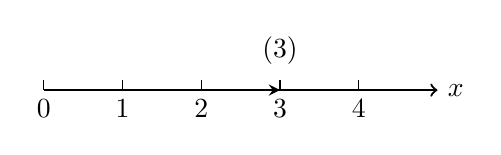
\begin{tikzpicture}
			\pgfmathsetmacro{\ticker}{0.125}
			 \draw [->,thick] (0,0) node (yaxis) [above] {}
							|- (5,0) node (xaxis) [right] {$x$};
			 \foreach \i/\texti  in {0,1,2,3,4} {
			 \draw (1*\i,0) --(1*\i,\ticker) node[label=below:\texti]{};
			 }
			 \draw[arrow] (0,0)--(3,0);
			 \node at (3,0.5) {$(3)$};
			\end{tikzpicture}
			\caption{一维向量示意图}
			\label{one_dimension_vector}
	\end{minipage}%
	\begin{minipage}[c]{0.5\textwidth}
	\centering
	 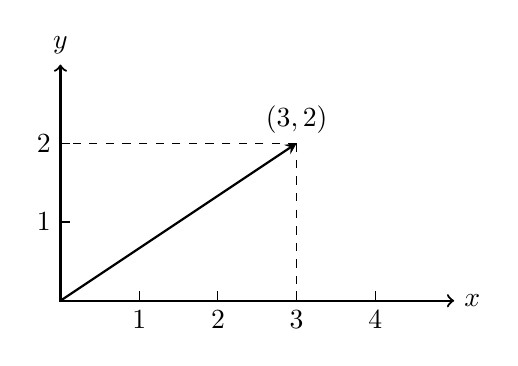
\begin{tikzpicture}
			\pgfmathsetmacro{\ticker}{0.125}
			\draw [<->,thick] (0,3) node (yaxis) [above] {$y$}
							|- (5,0) node (xaxis) [right] {$x$};
			\foreach \i/\texti  in {1,2,3,4} {
			\draw (1*\i,0) --(1*\i,\ticker) node[label=below:\texti]{};
			}
			\foreach \j/\textj  in {1,2} {
			\draw (0,1*\j) --(\ticker,1*\j) node[label=left:\textj]{};
			}
			\draw[arrow] (0,0)--(3,2);
			\draw[dashed] (3,2)--(3,0);
			\draw[dashed] (3,2)--(0,2);
			\node at (3,2.3) {$(3,2)$};
			\end{tikzpicture}
			\caption{二维向量示意图}
			\label{two_dimension_vector}
	\end{minipage}
	\end{figure}

向量指的是既包含大小,又包含方向的一类量,例如位移,速度,加速度,力等,又称为矢量。
在线性代数中,向量可以用矩阵的形式进行表示,例如一个一维的向量可以用向量$A=\left( \begin{array}{ccc}{a_{1}}\end{array}\right)$
表示,二维向量可以用$A=\left( \begin{array}{ccc}{a_{1},a_{2}}\end{array}\right)$表示,如图\ref{one_dimension_vector}和图\ref{two_dimension_vector}所示。
同理,我们可以推出,包含$n$个分量的向量可以称为$n$维向量,用
$A=\left( \begin{array}{ccc}{a_{1},a_{2},a_{3},\cdots,a_{n}}\end{array}\right)$表示。

\begin{figure}[!b]
	\begin{lstlisting}[language=Java]
		public static INDArray create(double[] data, long[] shape) {
	
			checkShapeValues(data.length, shape);
	
			INDArray ret = INSTANCE.create(data, shape, Nd4j.getStrides(shape, Nd4j.order()), DataType.DOUBLE, Nd4j.getMemoryManager().getCurrentWorkspace());
			return ret;
		}
	\end{lstlisting}
	\caption{NDArray的创建}
	\label{NDArray_creation}
\end{figure}

在DL4J中,普通矩阵的创建用create方法实现,源码如图\ref{NDArray_creation}所示。首先我们需要传入两个数组data和shape,
作为源数据组并决定矩阵的形状与维度。然后,系统会调用checkShapeValues方法
来确保输入data数组的长度与shape数组相符。最后,利用这些数据创建一个INDArray并返回,
这就完成了矩阵的创建。

特殊的,我们可以用简便的方法来创建部分简单的矩阵,例如zeros()方法可以创建一个全零矩阵,
仅需要传入行数和列数即可。同理还有ones(),valueArrayof()等方法。


\subsection{基本运算}

\begin{figure}[!ht]
	\centering
	\begin{minipage}[c]{0.5\textwidth}
	\centering
		\begin{equation*}
	    \left( \begin{matrix}
        a_{11} & a_{12} & \cdots & a_{1n}\\
        a_{21} & a_{22} & \cdots & a_{2n}\\
        \vdots & \vdots & \ddots & \vdots\\
        a_{m1} & a_{m2} & \cdots & a_{mn}
        \end{matrix}
        \right )
		\end{equation*}
		\caption{矩阵$A$}
		\label{matrix_a}
	\end{minipage}%
	\begin{minipage}[c]{0.5\textwidth}
	\centering
    \begin{equation*}
	    \left( \begin{matrix}
        b_{11} & b_{12} & \cdots & b_{1n}\\
        b_{21} & b_{22} & \cdots & b_{2n}\\
        \vdots & \vdots & \ddots & \vdots\\
        b_{m1} & b_{m2} & \cdots & b_{mn}
        \end{matrix}
        \right )
		\end{equation*}
		\caption{矩阵$B$}
		\label{matrix_b}
	\end{minipage}
\end{figure}

矩阵有四种运算:加减、数乘、乘法和转置。下面我们将用例子展示矩阵的运算,
假设我们有两个矩阵$A$和$B$,如图\ref{matrix_a}与图\ref{matrix_b}所示。

\subsubsection{矩阵的加减}

$A$和$B$是两个$m*n$型矩阵,那么存在矩阵$C$,记$C=A+B$,称$C$为矩阵$A$和$B$的加法运算。
需要注意的是,进行加法运算的两个矩阵行数和列数必须相等,否则无法进行运算。

\begin{figure}[!hb]
			\begin{equation*}
				\left( \begin{matrix}
					a_{11}+b_{11} & a_{12}+b_{12} & \cdots & a_{1n}+b_{1n}\\
					a_{21}+b_{21} & a_{22}+b_{22} & \cdots & a_{2n}+b_{2n}\\
					\vdots & \vdots & \ddots & \vdots\\
					a_{m1}+b_{m1} & a_{m2}+b_{m2} & \cdots & a_{mn}+b_{mn}
					\end{matrix}
					\right )
					\end{equation*}
			\caption{矩阵$C$}
\end{figure}

矩阵的加法在DL4J中由add方法和addi方法实现。代码会先检测输入的数组是否为数字矩阵,以此判断
是否可进行加法操作,最后将两个矩阵进行加法操作。


\begin{figure}[!hb]
	\begin{lstlisting}[language=Java]
		public INDArray add(INDArray other) {
	       validateNumericalArray("add", false);
		   return addi(other, Nd4j.createUninitialized(Shape.pickPairwiseDataType
		   (this.dataType(), other.dataType()), this.shape(), this.ordering()));}
	\end{lstlisting}
\end{figure}

\subsubsection{矩阵的数乘}

矩阵$A$是一个$m*n$型矩阵,$k$是一个数,则称矩阵$D$为矩阵$A$与数$k$的乘积,称为数乘,记为$kA$。

\begin{figure}[!h]
	\begin{equation}
		(ka_{ij})_{m*n}=
		\left( \begin{matrix}
			ka_{11} & ka_{12} & \cdots & ka_{1n}\\
			ka_{21} & ka_{22} & \cdots & ka_{2n}\\
			\vdots & \vdots & \ddots & \vdots\\
			ka_{m1} & ka_{m2} & \cdots & ka_{mn}
			\end{matrix}
			\right )
	\end{equation}
	\caption{矩阵$D$}
\end{figure}

矩阵的数乘与加法基本一致,都是先检验是否为数字矩阵的操作,随后对矩阵中的每个元素进行乘法操作。


\begin{figure}[!ht]
	\begin{lstlisting}[language=Java]
	  public INDArray mul(Number n) {
	     validateNumericalArray("mul", false);
		 return muli(n, Nd4j.createUninitialized(Shape.pickPairwiseDataType
		 (this.dataType(), n), this.shape(), this.ordering()));}
	\end{lstlisting}
	\end{figure}

矩阵的加法和数乘运算统称为矩阵的线性运算。矩阵的线性运算满足交换律,分配律和结合律。

\subsubsection{矩阵的乘法}

设$A=(a_{ik})_{m*s}$,$B=(b_{kj})_{s*n}$,定义$A$与$B$的乘积$AB$是一个$m*n$
矩阵$C=(C_{ij})_{m*n}$,$C$的第i行第j列元素等于$A$的第i行元素与$B$的第j列对应元素
乘积的代数和,如图\ref{matrix_e}:

\begin{figure}[!ht]
	\begin{equation*}
		AB=
		\left( \begin{matrix}
			a_{1}b_{1} & a_{1}b_{2} & \cdots & a_{1}b_{n}\\
			a_{2}b_{1} & a_{2}b_{2} & \cdots & a_{2}b_{n}\\
			\vdots & \vdots & \ddots & \vdots\\
			a_{n}b_{1} & a_{n}b_{2} & \cdots & a_{n}b_{n}
			\end{matrix}
			\right )
	\end{equation*}
	\caption{矩阵$E$}
	\label{matrix_e}
\end{figure}

DL4J中,矩阵乘法的源码先对进行乘法操作的两个矩阵判断是否为同一数据类型,之后再得出乘法计算后矩阵的
维度和形状,最后计算后将结果写入结果矩阵,返回结果,如图\ref{matrix_multiply_code}。


\begin{figure}[!ht]
	\begin{lstlisting}[language=Java]
		public INDArray mmul(INDArray other) {
			Preconditions.checkState(this.dataType() == other.dataType(), "Matrix multiplication: 
			    arrays must have same dtype: %s vs. %s", this.dataType(), other.dataType());
			long[] shape = {rows(), other.rank() == 1 ? 1 : other.columns()};
			INDArray result = createUninitialized(this.dataType(), shape, 'f');
			if (result.isScalar())
				return Nd4j.scalar(Nd4j.getBlasWrapper().dot(this, other)).reshape(1, 1);
			return mmuli(other, result);
		}
	\end{lstlisting}
	\caption{矩阵乘法源码}
	\label{matrix_multiply_code}
	\end{figure}


\subsubsection{矩阵的转置}

设存在$m*n$矩阵$A$,则称$n*m$矩阵$B$为$A$的转置矩阵,记为$A^T$。

\begin{figure}[!hb]
	\centering
	\begin{minipage}[c]{0.5\textwidth}
	\centering
		\begin{equation}
	    \left( \begin{matrix}
        a_{11} & a_{12} & \cdots & a_{1n}\\
        a_{21} & a_{22} & \cdots & a_{2n}\\
        \vdots & \vdots & \ddots & \vdots\\
        a_{m1} & a_{m2} & \cdots & a_{mn}
        \end{matrix}
        \right )
        \end{equation}
		\caption{矩阵$A$}
	\end{minipage}%
	\begin{minipage}[c]{0.5\textwidth}
	\centering
    \begin{equation}
	    \left( \begin{matrix}
        a_{11} & a_{21} & \cdots & a_{m1}\\
        a_{12} & a_{22} & \cdots & a_{m2}\\
        \vdots & \vdots & \ddots & \vdots\\
        a_{1n} & a_{2n} & \cdots & a_{mn}
        \end{matrix}
        \right )
        \end{equation}
		\caption{矩阵$B$}
	\end{minipage}
\end{figure}

在DL4J中,矩阵的转置调用了permute方法,先将原矩阵的形状,源数据,排列规则等属性提出并进行转置,
再利用新属性生成一个新的INDArray并返回,在实际使用中我们需要调用transpose()方法即可
完成矩阵的转置。

\begin{figure}[!ht]
	\begin{lstlisting}[language=Java]
		public INDArray permute(int... rearrange) {
	
	       checkArrangeArray(rearrange);
	       int[] newShape = doPermuteSwap(shapeOf(), rearrange);
	       int[] newStride = doPermuteSwap(strideOf(), rearrange);

	       char newOrder = Shape.getOrder(newShape, newStride, 1);

	       INDArray value = create(data(), newShape, newStride, offset(), newOrder);
				 return value;
		}
	\end{lstlisting}
\end{figure}

\subsection{多维空间}

多维空间一般指多维向量空间。一般来说,我们将实数域上的全体$n$维向量构成的集合称为$n$维向量
空间$R^n$。

在此基础上,我们设$\alpha_{1},\alpha_{2},\alpha_{3}...,\alpha_{r}$是向量空间中$V$
中的向量,若它们满足:(1)$\alpha_{1},\alpha_{2},\alpha_{3}...,\alpha_{r}$线性无关;
(2)$V$中的任何一个向量都可以用$\alpha_{1},\alpha_{2},\alpha_{3}...,\alpha_{r}$线性
表示,则称$\alpha_{1},\alpha_{2},\alpha_{3}...,\alpha_{r}$为向量空间$V$的一个基,
$r$称为向量空间$V$的维数,并称$V$为$r$维向量空间。

显然,向量空间的基不是唯一的。同时,我们应该注意到向量的维数和向量空间的维数并不是同一个概念。




\subsection{特征值与特征向量}

设$A$是一个$n$阶矩阵,如果存在数$\lambda$和非零列向量$\alpha$,使得$A\alpha=\lambda\alpha$,
则称$\lambda$为矩阵$A$的一个特征值,称$\alpha$为$A$属于特征值$\lambda$的一个特征向量。

\vspace{5pt}

\begin{figure}[!ht]
	\begin{lstlisting}[language=Java]
		private static void getEigenValue(int[] A){
			int a = 1;
			int b = -(A[0] + A[3]);
			int c = A[0]* A[3] - A[1] * A[2];
			double t = b*b - 4 * (a * c);
			if (t >= 0) {
				double lambda1 = (Math.sqrt(t) - b) * 1.0 / (2 * a);
				double lambda2 = (-(Math.sqrt(t))-b) * 1.0 / (2 * a);
				int[] resultArray1 = {1,(int)((A[2])/(lambda1 - A[3]))};
				System.out.print("矩阵的第一个特征值为" + lambda1 + ",特征向量为" + "[" + resultArray1[0] 
				+ "," + resultArray1[1] + "]");
			}
	  }
	\end{lstlisting}
\end{figure}

代码块展示了简单的二维矩阵计算特征值与特征向量的方法。在此过程中,我们首先求出矩阵$A$的特征多项式,
并求出$A$的所有特征值;然后再根据特征值求出齐次线性方程组$(\lambda*I-A)x=0$的基础解系,进而
得出特征向量。

\section{雅克比矩阵}

雅克比矩阵是一阶偏导数以一定方式排列组成的矩阵。在线性代数中,
雅克比矩阵体现了一个可微方程与给定点的最优线性逼近,有着重要的意义。

雅克比矩阵的定义为假设存在$n$个$y_n=f(x_1,x_2,...,x_n)$型函数。如果这些函数的偏导数存在,则可组成一个$m$行$n$列的矩阵,
这个矩阵就是雅克比矩阵,用符号表示为$J_F(x_1,...,x_n)$,如图\ref{jacobin_matrix}所示。

\begin{figure}[!hb]
	\begin{equation}
		J_F(x_1,...,x_n)=
		\left( \begin{matrix}
			\frac{\partial y_1}{\partial x_1} & \cdots & \frac{\partial y_1}{\partial x_n}\\
			\vdots & \ddots & \vdots\\
			\frac{\partial y_m}{\partial x_1} & \cdots & \frac{\partial y_m}{\partial x_n}
			\end{matrix}
			\right )
	\end{equation}
	\caption{雅克比矩阵}
	\label{jacobin_matrix}
\end{figure}



\section{Hessian矩阵}

Hessian矩阵又称黑塞矩阵,海瑟矩阵。与雅克比矩阵相对应,是多元函数的二阶偏导数构成的
方阵,描述了函数的局部曲率情况。

Hessian矩阵的定义为设有一个$n$元实函数$f(x_1,x_2,...,x_n)$在定义域内有二阶连续偏导,
这些二阶偏导组成的矩阵被称为Hessian矩阵,如下图所示。

\begin{figure}[!h]
	\begin{equation}
		\left( \begin{matrix}
			\frac{\partial^2 f}{\partial x_1^2} & \frac{\partial^2 f}{\partial x_1 \partial x_2} & \cdots & \frac{\partial^2 f}{\partial x_1 \partial x_n}\\
            \frac{\partial^2 f}{\partial x_2^2} & \frac{\partial^2 f}{\partial x_2 \partial x_2} & \cdots & \frac{\partial^2 f}{\partial x_2 \partial x_n}\\
			\vdots & \vdots & \ddots & \vdots\\
			\frac{\partial^2 f}{\partial x_n^2} & \frac{\partial^2 f}{\partial x_n \partial x_2} & \cdots & \frac{\partial^2 f}{\partial x_n^2}
			\end{matrix}
			\right )
	\end{equation}
	\caption{Hessian矩阵}
\end{figure}


\section{泰勒展开和牛顿法}
在数学中,泰勒展开式主要指利用函数在一点的各阶导数值,
来构建一个多项式近似函数值,同时还能给出近似值与实际值的误差。
如果一个函数在点$x_0$处可以计算$n$阶导数,则我们有Taylor展开:

\begin{equation*}
	f(x)=f\left(x_{0}\right)+f^{\prime}\left(x_{0}\right)\left(x-x_{0}\right)+\frac{f^{\prime \prime}\left(x_{0}\right)}{2 !}\left(x-x_{0}\right)^{2}+\cdots+\frac{f^{(n)}\left(x_{0}\right)}{n !}\left(x-x_{0}\right)^{n}+R_{n}(x)
\end{equation*}

其中$R_n(x)$称为拉格朗日余项,值为$R_{n}(x)=\frac{f^{(n+1)}(\xi)}{(n+1) !}\left(x-x_{0}\right)^{n+1}$,
当$x_0=0$时,我们能得到Taylor的麦克劳林公式:

\begin{equation*}
	f(x)=f(0)+f^{\prime}(0) x+\frac{f^{\prime \prime}(0)}{2 !} x^{2}+\cdots+\frac{f^{(n)}(0)}{n !} x^{n}+o\left(x^{n}\right)
\end{equation*}


\section{向量与矩阵求导}

利用向量和矩阵求导可以让原本有许多变量的单个函数的偏导值收集到可以视为单个个体的矩阵和向量
当中,这大大简化了我们寻找多元函数的最大值或最小值,微分方程组操作等问题。

在上面的两节里,我们介绍了雅克比矩阵和Hessian矩阵,它们的本质都是特殊的矩阵求导。
在这里我们将给出一般的形式。对于一个向量$y=(y_{1},y_{2},...,y_{m})$对
x求导,我们可以写成$\frac{\partial y}{\partial x}=\left( \begin{array}{ccc}{\frac{\partial y_{1}}{\partial x},\frac{\partial y_{2}}{\partial x},
...,\frac{\partial y_{m}}{\partial x}}\end{array}\right)$。在求解梯度下降的加速度问题
时,向量求导能比较好地解决问题。矩阵的求导与雅克比矩阵的形式十分类似,都是对矩阵中的元素逐个求导。

同理,矩阵的求导也与此类似,设有函数矩阵$Y$,其对于$x$的求导结果可以表示为:

\begin{figure}[!h]
	\begin{equation}
		J_F(x_1,...,x_n)=
		\left( \begin{matrix}
			\frac{\partial y_{11}}{\partial x} & \cdots & \frac{\partial y_{1n}}{\partial x}\\
			\vdots & \ddots & \vdots\\
			\frac{\partial y_{m1}}{\partial x} & \cdots & \frac{\partial y_{mn}}{\partial x}
			\end{matrix}
			\right )
	\end{equation}
	\caption{矩阵的求导}
\end{figure}



\chapter{数学基础-DEMO}
\label{chap:math_regression}

\gls{AI}实在是一个多学科综合性应用,涉及到的理论不仅多而且深。限于笔者知识水平以及篇幅要求,不会对此进行长篇巨幅地解释。


\section{向量运算}
单独的一个数字,称为\emph{标量}(scalar),而向量通常用数组的形式表示。一个\emph{向量}就是一列(行)数字:
\begin{equation}
x=[x_1 x_2 \dots x_n],
x=\left[\begin{array}{c} x_1\\x_2\\\dots\\x_n\end{array}\right]
\label{part2_vector_form}
\end{equation}
\ \\
向量是一种带方向指示性的量,代表空间中的一个点。一维向量$\vec{a}=\left[4\right]$代表a点在原点右侧距离为4的位置。
而二维向量$\vec{b}=\left[3\ 4\right]$就代表了在第一象限坐标(3,4)有一个点b。所以,向量是一个方向性的偏移量。
\emph{向量}可以在坐标系中自由平移,选定一个起点就确定了它的终点。

\begin{center} \begin{tikzpicture}
\node[circle,draw,black,scale=0.2] (A) at (1,2) {};
\node[circle,draw,black,scale=0.2] (B) at (3,4) {};
\draw[arrow]
    (A)node[below]{A起点}--(B)node[above]{B终点};
\end{tikzpicture}\end{center} 

向量支持的运算有\emph{内积}(点乘)和\emph{外积}(叉乘)运算,以及加减运算。
向量A、B的运算过程,设$\vec{A} = (a1,  a2,  a3), \vec{B} = (b1,  b2,  b3)$

\begin{itemize}
\item[1.] 点乘,结果是一个标量:$A \cdot B = a1*b1 + a2*b2 + a3*b3$
\item[2.] 叉乘,结果还是个向量:$A \times B = (a2*b3 - a3*b2, a3*b1 - a1*b3, a1*b2 - a2*b1)$
\item[3.] 标量,用于每一个元素:$A + 2 = (a1+2, a2+2, a3+2)$
\end{itemize}

\noindent
通常使用\emph{数组}来表示向量,但这样扩展性不够好。咱们使用Java面向对象的方法,把数组和函数封装进一个向量类型里面去。定义一个Vector类,如\figref{fig:part2_math_vector}:

\begin{figure}[!htb]
\begin{center}\begin{tikzpicture}
\umlclass[y=-3]{InVector}{
    array : int[] 
}{
    add(v : InVector) : InVector \\
    sub(v : InVector) : InVector \\
    dot(v : InVector) : int \\
    cross(v : InVector) : IntVector
}
\label{fig:part2_math_vector}
\end{tikzpicture}\end{center}
\caption{类图:IntVector}
\end{figure}

\begin{lstlisting}[language=Java]
public IntVector(int... array) {
    this.array = array;
}

public IntVector add(IntVector vector) {
    foreach(this.array, vector.array, (a,b)->a+b);
    return this;
}

public int dot(IntVector vector) {
    return foreach(this.array, vector.array, (a,b)->a*b);
}
\end{lstlisting}

\noindent
如上代码,构造函数用到了可变参数,你可以理解成一个\lstinline{int[]}。在编译的时候,Java会自动地把函数声明和调用代码都转换成数组。
\emph{add}运算返回\lstinline{this},用来支持链式运算:$v1.add(v2).add(v3)\dots$。容易看出,
\emph{add}和\emph{dot}运算,是对应元素相加、相乘的过程。
使用\emph{foreach}从相加的2个向量中,逐个地取出数据并执行$\lambda$操作。\\

\begin{lstlisting}[language=Java,caption=叉乘运算]
public IntVector cross(IntVector vector) {
    int[] v1 = this.array;
    int[] v2 = vector.array;

    int length = vector.array.length;
    if (length == 2) {
        return new IntVector(v1[0]*v2[1]-v1[1]*v2[0]);
    }

    int[] result = IntStream.range(0, length).map(
        i->v1[(i+1)%length]*v2[(i+2)%length] -v1[(i+2)%length]*v2[(i+1)%length]
    ).toArray();

    return new IntVector(result);
}

// sum用于dot运算
private static int foreach(int[] src, int[] dst, IntBinaryOperator op) {
    int sum = 0;
    for (int i = 0; i < src.length; i++) {
        src[i] = op.applyAsInt(src[i], dst[i]);
        sum += src[i];
    }
    return sum;
}
\end{lstlisting}

以上,仅仅只能处理int类型的向量。
结合IntVector的实现代码,相信大家也能理解实数类型的向量。
也许你也意识到,使用\emph{add}太麻烦了,但Java目前还不支持运算符重载。
如果确实想使用,可以借助\emph{Java-OO开源插件}\footnote{一种使用APT在编译过程中替换运算符为相应函数的方法。}
\vspace{0.3cm}

\begin{lstlisting}[language=Java, caption=运算符重载]
@Test
public void add_operator_override() {
    IntVector a = new IntVector(1,2,3);
    IntVector b = new IntVector(10,20,30);

    IntVector c = a + b; // 看上去运算符重载了
    int[] expected = new int[]{11, 22, 33};

    assertArrayEquals(expected, c.array);
    assertEquals(new IntVector(expected), c);
}
\end{lstlisting}

实际上,很少有自己实现的,并且也较难保障准确性和稳定性。开源的ND4J作为DL4J的张量计算库,提供了丰富的运算接口,支持几乎所有的数学操作,相当于Python界的numpy。以下\coderef{code:part2_math_dl4j}

\begin{lstlisting}[language=Java,caption={dl4j例子},label=code:part2_math_dl4j]
INDArray vec1 = Nd4j.create(new float[]{1,2,3});

// vector add
INDArray vec2 = Nd4j.create(new float[]{10,20,30});

// [[11.0000, 22.0000, 33.0000]]
System.out.println(vec1.add(vec2));

// scalar add
INDArray vec3 = vec1.add(10);

// [[11.0000, 12.0000, 13.0000]]
System.out.println(vec3);
\end{lstlisting}

ND4J在开源、分布式、支持GPU的库内,为Java带来了符合直觉的,类似Python编程人员所用的科学计算工具。
它具有:
\begin{itemize}
\item[1.] 多用途多维数组对象
\item[2.] 多平台功能,包括GPU
\item[3.] 线性代数和信号处理功能
\end{itemize}

\noindent
本节之后都将使用ND4J来演示算法,有兴趣的同学可以研究它的实现代码。

\section{矩阵运算}

矩阵是一个$m \times n$个数组成的m行n列的矩形表格。
特别地,向量可以看作矩阵的特殊形式。
对于$1 \times n$或$n \times 1$的矩阵,就是一个行向量或列向量。
实际上,矩阵的\emph{加法/减法}运算,也可适用于向量。
尽管矩阵是多维度数据,却很少采用多维数组表示。
如果\emph{向量}和\emph{矩阵}都使用一维数组表示的话,\emph{add}运算当然可以用与矩阵。

\vspace{0.3cm}\noindent
对于这样一个数组: \lstinline|int[] numbers={1,2,3,4,5,6}|。
\begin{itemize}
\item[1.] 可能是一个$1 \times 6$的矩阵,或是一个向量。
\item[2.] 可能是一个$2 \times 3$的矩阵
\item[3.] 可能是一个$3 \times 2$的矩阵
\end{itemize}

\begin{figure}[!htb]
\begin{center}\begin{tikzpicture}
\umlclass[y=-3]{IntNDArray}{
    array : int[] \\
    shape : int[]
}{
    add(v : IntNDArray) : IntNDArray \\
    mul(v : IntNDArray) : IntNDArray \\
    rank(): int \\
    isVector(): boolean
}
\label{fig:part2_math_matrix}
\end{tikzpicture}\end{center}
\caption{类图:IntNDArray}
\end{figure}

为了让IntVector升级为IntNDArray,势必要加入维度信息才行,记为\emph{shape}。而矩阵只有2个维度,如果不考虑更多维度的情况下,
使用\lstinline|int[2]|就可以。但你立即就会认识到,改成\lstinline|int[]|有更好的可扩展性。
使用\emph{IntNDArray}创建向量就是创建$1 \times n$或$n \times 1$的矩阵。

\begin{lstlisting}[language=Java,caption={创建NDArray}]
int[] array;
int[] shape;

// 默认:1 x n
public IntNDArray(int... array) {
    this.array = array;
    this.shape = new int[]{1, array.length};
}

// 可以把1x6转换成2x3或者3X2的矩阵
public IntNDArray reshape(int[] shape) {
    this.shape = shape;
    return this;
}
\end{lstlisting}

根据数学定义,只有当矩阵A的列数等于矩阵B的行数时,A与B才可以相乘。乘积C的第m行第n列的元素等于矩阵A的第m行的元素与矩阵B的第n列对应元素乘积之和。

\begin{equation}
c_{ij}= \sum_{k=1}^pa_{ik}*b_{kj}
\end{equation}
其中,A为m $\times$ p的矩阵,B为p $\times$ n,结果为mxn的矩阵C。
相应地,实现算法如下:

\begin{lstlisting}[language=Java,caption={矩阵乘法}]
public IntNDArray mul(IntNDArray ndArray) {
    final int ROWS = this.shape[0];
    final int COLS = ndArray.shape[1];

    int[] shape = new int[]{ROWS, COLS};
    int[] data = new int[ROWS*COLS];

    for(int i=0; i<ROWS; i++) {
        for (int j=0; j<COLS; j++) {
            for (int k=0; k<ndArray.shape[0]; k++) {
                int a_i_k = this.array[i*this.shape[1]+k];
                int b_k_j = ndArray.array[k*ndArray.shape[1]+j];
                data[i*COLS+j] += a_i_k * b_k_j;
            }
        }
    }
    return new IntNDArray(data).reshape(shape);
}
\end{lstlisting}

现在,我们就可以用一维数组记录矩阵了,不管维度如何变化reshape之后不需要变更array的内容。
对于\emph{向量}的点乘和叉乘,也可以借助\emph{矩阵}处理。
\emph{点乘}比较容易解决,但\emph{叉乘}需要\emph{反对称}矩阵(anti-symmetric)辅助才能计算出结果。
不过\emph{叉乘}主要应用于几何和动量计算,在此就不再详细解释。

\vspace{0.3cm}\noindent
以下代码是ND4J的矩阵示例:
\begin{lstlisting}[language=Java]
INDArray v1 = Nd4j.create(new float[]{1,2,3}).reshape(1,3);
INDArray v2 = Nd4j.create(new float[]{10,20,30}).reshape(3,1);
System.out.printf("v1v2=[%s]\n", v1.mmul(v2));
\end{lstlisting}


\section{梯度下降}
在机器学习里,梯度下降虽然不是什么高深的算法,但它却是机器学习的关键。经常会用到梯度下降法来进行训练,常见的有:
批量梯度下降法BGD,随机梯度下降法SGD,小批量梯度下降法MBGD。

\begin{figure}[!htb]
\centerline{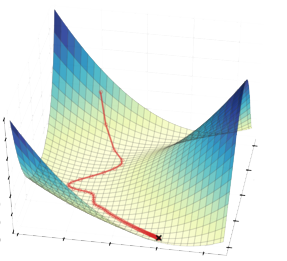
\includegraphics[width=.2\figwidth]{images/sgd.png}}
\label{fig:part2_math_sgd}
\caption{梯度下降}
\end{figure}

梯度是方向上升/下降最快的方向,它的幅值代表陡峭的程度。
所以,在最小值的地方,曲面轮廓几乎是平坦的,理论上最小值是梯度为0。
但事实上,我们又可能无法达到最小值,只能在最小值附近的平坦区域来回震荡。
当在这个区域震荡时,损失(Loss)值几乎是我们能达到的最小值了,并且不会有很大的变化,因此我们是在真实的最小值附近跳动。
通常,当损失值在预定的数字内没有改善的时候就会停止迭代,例如10次或者20次迭代。
当这种情况发生时,就说训练已经收敛了,或者说收敛已经完成了。

\subsection{BGD}
使用BGD(Batch Gradient Descent,批量梯度下降),在目标函数为凸函数时,虽然可以找到全局最优解,
但收敛速度慢,需要用到全部数据,因此内存消耗也大。因此,BGD不适用于大数据集。
其公式如下:

\noindent
$$\boldsymbol{W} \leftarrow \boldsymbol{W}-\eta \frac{\partial \boldsymbol{L}}{\partial \boldsymbol{W}}$$

\noindent
如公式所示,BGD的策略就是朝着当前所在位置的坡度最大的方向前进。
但它也有缺点,它在面对峡谷型函数时,效率会变得很低,呈现出震荡的姿态。

\subsection{SGD}
而SGD相当于BGD的升级版。SGD被称为随机梯度下降(Stochastic Gradient Desccent)。
正如它的名字所说,它首先通过mini-batch学习,
意思就是从训练数据中随机选择一部分数据(称为mini-batch),
将这些mini-batch作为对象,使用梯度法进行学习。
其代码如下所示:


\begin{lstlisting}[language=java]
	MultiLayerConfiguration conf = new NeuralNetConfiguration.Builder()
        .weightInit(WeightInit.XAVIER)
        .activation("relu")
        .optimizationAlgo(OptimizationAlgorithm.STOCHASTIC_GRADIENT_DESCENT)
        .updater(new Sgd(0.05))
        // ... other hyperparameters
        .list()
        .backprop(true)
        .build();
\end{lstlisting}


\subsection{Momentum}
Momentum也是一种常见的优化算法,也被称为SGD with Momentum。
恰如其名,它为了抑制SGD的震荡,在梯度下降过程中加入惯性。
简单来说,它就是在梯度越陡时,下降越快。较平缓时,下降较慢。
其公式如下:

$$\boldsymbol{v} \leftarrow \alpha \boldsymbol{v}-\eta \frac{\partial \boldsymbol{L}}{\partial \boldsymbol{W}}$$

$$\boldsymbol{W} \leftarrow \boldsymbol{W}+\boldsymbol{v}$$

\noindent
如上式所示,$\boldsymbol{W}$表示要更新的权重参数,$\frac{\partial L}{\partial \boldsymbol{W}}$
表示损失函数关于$\boldsymbol{W}$的梯度,$\eta$表示学习率。
而$\boldsymbol{v}$这一变量便是用来模拟惯性的。
其通过在SGD的基础上引入一阶动量,
这代表着现在下降方向不仅由当前点的梯度方向决定,而且由此前累积的下降方向决定。 


\begin{lstlisting}[language=java]
	MultiLayerConfiguration conf = new NeuralNetConfiguration.Builder()
        .weightInit(WeightInit.XAVIER)
        .activation("relu")
        .optimizationAlgo(OptimizationAlgorithm.STOCHASTIC_GRADIENT_DESCENT)
        .updater(new Nesterovs(0.05))
        // ... other hyperparameters
        .list()
        .backprop(true)
        .build();
\end{lstlisting}

\noindent
Momentum的更新路径就如同小球在碗中滚动一样。
与SGD相比,其大大缓解了震荡问题,原因就是它加入的一阶动量。
即使在某一方向“受力”很小,但因为其一直在同一方向受力,
所以它会朝着同一方向有一定的加速。
通俗地讲,就是它所加入的惯性,抵消了试图改变它的力。

\subsection{AdaGrad}
在梯度下降中,学习率的值很重要(记为$\eta$),
而在学习率的相关研究中,有一种被称为\textbf{学习率衰减}(learning rate decay)的方法,
随着机器学习的过程,使学习率逐渐减小。
它具体表现为,在一开始与其他方法类似,进行参数学习,
但在学习的过程中,当准确率越来越高时,便减少学习率。
其公式如下:
$$\boldsymbol{h} \leftarrow \boldsymbol{h}+\frac{\partial \boldsymbol{L}}{\partial \boldsymbol{W}} \odot \frac{\partial \boldsymbol{L}}{\partial \boldsymbol{W}}$$

$$\boldsymbol{W} \leftarrow \boldsymbol{W}-\eta \frac{1}{\sqrt{\boldsymbol{h}}} \frac{\partial \boldsymbol{L}}{\partial \boldsymbol{W}}$$

如公式所示,AdaGrad会为参数的每个元素适当地调整学习率,
与此同时进行参数的学习。AdaGrad的公式比起之前的,
新出现了一个变量$\boldsymbol{h}$,它代表着之前所有梯度值的平方和,
在更新参数时,通过乘以$\frac{1}{\sqrt{\boldsymbol{h}}}$,
AdaGrad便可以为每个元素调整适宜它的学习率。其代码如下所示:

\begin{lstlisting}[language=java]
	MultiLayerConfiguration conf = new NeuralNetConfiguration.Builder()
        .weightInit(WeightInit.XAVIER)
        .activation("relu")
        .optimizationAlgo(OptimizationAlgorithm.STOCHASTIC_GRADIENT_DESCENT)
        .updater(new AdaGrad(0.05))
        // ... other hyperparameters
        .list()
        .backprop(true)
        .build();
\end{lstlisting}
AdaGrad比起Momentum更好地抑制了SGD的震荡,函数的取值高效地向着最小值移动。
刚开始时,也许还会有些震荡,但越接近最小值,几乎是呈直线般向着目标前进。

\subsection{Adam}

\begin{lstlisting}[language=java]
	MultiLayerConfiguration conf = new NeuralNetConfiguration.Builder()
        .weightInit(WeightInit.XAVIER)
        .activation("relu")
        .optimizationAlgo(OptimizationAlgorithm.STOCHASTIC_GRADIENT_DESCENT)
        .updater(new Adam(0.05))
        // ... other hyperparameters
        .list()
        .backprop(true)
        .build();
\end{lstlisting}




\section{概率分布}

\section{损失函数}
在机器学习中,机器的学习需要某个指标来表示现在的状态,然后,以这个指标为基准,寻找最优权重参数。
而在机器学习中所用的指标便被称为\emph{损失函数}(loss function)。
对于损失函数,我们主要使用均方误差和交叉熵误差。

首先,我们介绍一种常用的函数,\emph{交叉熵误差}(cross entropy error)。
\begin{equation}
    E = - \sum _ { k } t _ { k } \log y _ { k }
    \label{part2_cross_entropy_error_1}
\end{equation}

在上式中,$y_{k}$代表着机器学习的输出,log表示以e为底数的自然对数($log_{e}$)。
$t_{k}$代表着正确解标签,仅当解标签为正确时,$t_{k}$的索引才为1。其余情况都为0。
因此,E所代表的实际为解标签为正确时所输出的自然对数。

%交叉熵误差的图像

如上图所示,当输出结果$y_{k}$越发趋向于1.0时,得到的E越发增大而趋向于0。
交叉熵误差通过E所表示的负值,来表明该权重参数与正确结果之间的偏差程度。

下面,我们用代码来实现交叉熵误差:
%代码
\begin{lstlisting}[language=Java,caption={交叉熵误差}]
\end{lstlisting}

%代码分析

%实际运行

\ \\
下面我们介绍另一种,在损失函数中最有名的\emph{均方误差}(mean squared error)。
它的公式如下所示:

\begin{equation}
    E = \frac { 1 } { 2 } \sum _ { k } \left( y _ { k } - t _ { k } \right) ^ { 2 }
    \label{part2_cross_entropy_error_2}
\end{equation}

在上式中k表示着数据处于哪一个维度,$t_{k}$表示着各维度的监督数据。通常情况下,
监督数据仅将正确解标签表示为1,而其他非正确解则表示为0。
而机器学习输出的结果$y_{k}$,则是会在各个维度都显示该维度是正确解标签的可能性。
均方误差通过计算机器学习的输出和正确解监督数据的各个元素之差的平方,再求总和。
从而得到该权重参数的输出结果与正确结果之间的偏差。

%代码
\begin{lstlisting}[language=Java,caption={均方误差}]
\end{lstlisting}

%代码分析

%实际运行

\section{拟合算法}

很多时候,我们希望通过一些样本来反应总体的特征,因此我们需要拟合曲线来判断总体的情况。 
假设有如下这些个样本,看起来各点分布趋于一条直线,因此我们希望通过一条直线来描述该样本所在总体的一些特征,对总体进行预测。一般的方法就是先假设一条直线,如L=ax+b,之后再根据前面这些样本,确定最优的a,b,所谓最优就是通过这些点计算出合适的a,b,使各个点对直线上垂直距离的平方和最小(最小二乘法)。具体的方法是通过迭代来计算的。













\chapter{机器学习}
\label{chap:machinelearning}

\section{分类问题}
分类问题就是将数据以一定的分类标准分为几簇,在本节中,我们将介绍几种分类方法。
第一种分类方法是SVM(Support Vector Machine,支持向量机),是机器学习中经典的算法。
我们以简单的逻辑分类为例,如图\ref{SVM_picture}所示,我们需要找到一条直线,这样就能将所有的数据分为两类。

\begin{figure}[!ht]
    \begin{center}
    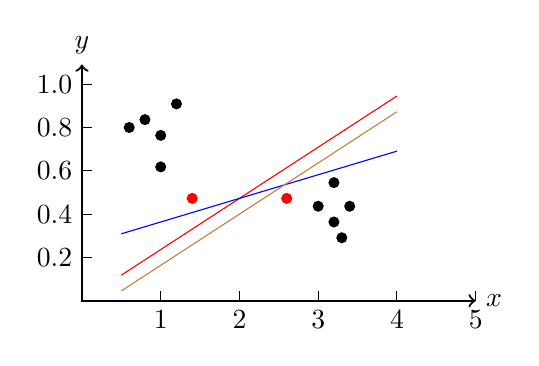
\begin{tikzpicture}
        \pgfmathsetmacro{\ticker}{0.125}
        \draw [<->,thick] (0,3) node (yaxis) [above] {$y$}
                |- (5,0) node (xaxis) [right] {$x$};
        \foreach \i/\texti  in {1,2,3,4,5} {
        \draw (1*\i,0) --(1*\i,\ticker) node[label=below:\texti]{};
        }
        \foreach \j/\textj  in {0.2,0.4,0.6,0.8,1.0} {
        \draw (0,2.75*\j) --(\ticker,2.75*\j) node[label=left:\textj]{};
        }
        \fill[black] (1,1.7) circle (2pt);
        \fill[black] (0.6,2.2) circle (2pt);
        \fill[black] (0.8,2.3) circle (2pt);
        \fill[black] (1,2.1) circle (2pt);
        \fill[black] (1.2,2.5) circle (2pt);
        \fill[red] (1.4,1.3) circle (2pt);
        
        \fill[black] (3.2,1) circle (2pt);
        \fill[black] (3,1.2) circle (2pt);
        \fill[black] (3.2,1.5) circle (2pt);
        \fill[black] (3.3,0.8) circle (2pt);
        \fill[black] (3.4,1.2) circle (2pt);
        \fill[red] (2.6,1.3) circle (2pt);
        
        \draw[color=red, domain=0.5:4]    plot (\x,{0.65 * \x}) node[right]{};
        \draw[color=blue, domain=0.5:4]    plot (\x,{0.3 * \x + 0.7}) node[right]{};
        \draw[color=brown, domain=0.5:4]  plot(\x,{0.65 * \x - 0.2}) node[right] {};
        \end{tikzpicture}
        \caption{支持向量机示意图}
        \label{SVM_picture}
    \end{center}
    \end{figure}


如果不加以限制,这样的分类直线将有无数条。
为了在众多的直线中找到最优的分类直线,我们要遵循间隔最大化原则,
即分类直线离数据越远就是最优的,因为如果不是这样,
分类直线会紧贴边界的数据;这时如果出现一个与边界数据略有不同的新数据,
就很容易被分到错误的一边。同时,过于接近分类直线的数据点不具有太大的实际意义。
想要达到分类直线离数据最远的效果,我们需要找到离分类直线最近的数据点,
用它们与直线的距离来训练神经网络。这些数据点被称为支持向量,这也是支持向量机名字的由来。

还是以图\ref{SVM_picture}为例,图中两个红色的点为支持向量,也就是离分类直线最近的两个点。
蓝线因为离两个支持向量都不是最远,所以不是最佳分类直线;棕线离上方的支持向量足够远,
然而最佳分类直线应与所有支持向量保持最远距离,
即所有支持向量离直线等距且最远,所以棕线也不符合要求。红线符合上述所有要求,
时这个数据集的最佳分类直线。

分类问题的第二种分类方法是RBM(Restricted Boltzmann Machine,受限波兹曼机)。
RBM是一种无向图模型,具有两层结构:可见层(V层),隐藏层(H层),这两层的节点相互全部连接,
但是每一层各自的神经元之间没有连接,因此被称为受限波兹曼机。波兹曼机是允许同一层神经元连接的。



\begin{figure}
    \begin{center}
    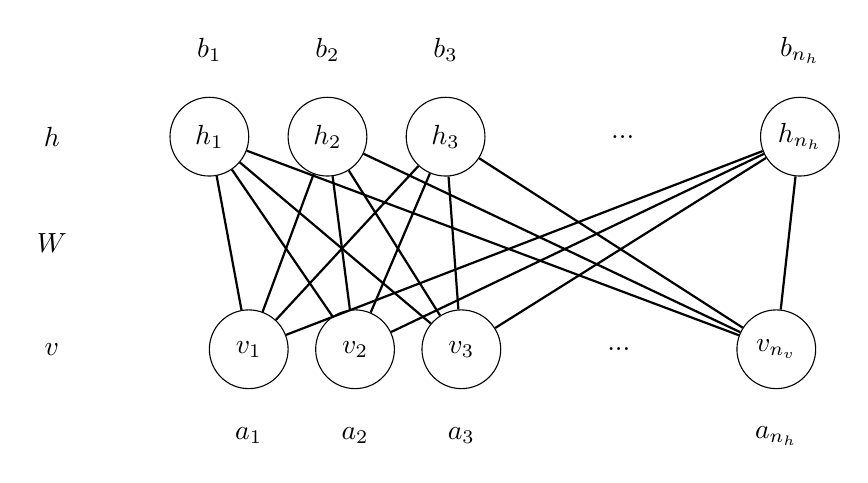
\begin{tikzpicture}
    \tikzstyle{arrow} = [thick, -, >= stealth]
    \tikzstyle{node} = [circle,  minimum width = 1cm, minimum height=1cm ,text centered, draw = black]
    \node[](H){$h$};
    \node[node, right of = H, xshift = 1cm](H1){$h_1$};
    \node[node, right of = H1, xshift = 0.5cm](H2){$h_2$};
    \node[node, right of = H2, xshift = 0.5cm](H3){$h_3$};
    \node[right of = H3, xshift = 1.25cm](...){...};
    \node[node, right of = ..., xshift = 1.25cm](Hn){$h_{n_h}$};

    \node[below of = H, yshift = -0.35cm](W){$W$};

    \node[below of = H, yshift = -1.7cm](V){$v$};
    \node[node, right of = V,xshift = 1.5cm](V1){$v_1$};
    \node[node, right of = V1, xshift = 0.35cm](V2){$v_2$};
    \node[node, right of = V2, xshift = 0.35cm](V3){$v_3$};
    \node[right of = V3, xshift = 1cm](...1){...};
    \node[node, right of = ...1, xshift = 1cm](Vn){$v_{n_v}$};
    
    \node[above of = H1, yshift = 0.1cm](b1){$b_1$};
    \node[above of = H2, yshift = 0.1cm](b2){$b_2$};
    \node[above of = H3, yshift = 0.1cm](b3){$b_3$};
    \node[above of = Hn, yshift = 0.1cm](bn){$b_{n_h}$};
    
    \node[below of = V1, yshift = -0.1cm](a1){$a_1$};
    \node[below of = V2, yshift = -0.1cm](a2){$a_2$};
    \node[below of = V3, yshift = -0.1cm](a3){$a_3$};
    \node[below of = Vn, yshift = -0.1cm](an){$a_{n_h}$};

    \draw[arrow] (H1)--(V1);
    \draw[arrow] (H1)--(V2);
    \draw[arrow] (H1)--(V3);
    \draw[arrow] (H1)--(Vn);
    \draw[arrow] (H2)--(V1);
    \draw[arrow] (H2)--(V2);
    \draw[arrow] (H2)--(V3);
    \draw[arrow] (H2)--(Vn);
    \draw[arrow] (H3)--(V1);
    \draw[arrow] (H3)--(V2);
    \draw[arrow] (H3)--(V3);
    \draw[arrow] (H3)--(Vn);
    \draw[arrow] (Hn)--(V1);
    \draw[arrow] (Hn)--(V2);
    \draw[arrow] (Hn)--(V3);
    \draw[arrow] (Hn)--(Vn);

    \end{tikzpicture}
    \caption{受限波兹曼机模型结构}
    \label{SVM_model_picture}
    \end{center}
\end{figure}


另外,受限波兹曼机是二值化的,也就是说,其神经元的输出只有两种状态:激活和未激活,
一般情况下我们分别用1和0表示。在图\ref{SVM_model_picture}所示的例子中,$n_v$和$n_h$分别表示可见层和隐藏层的神经元数目;
前面我们提到,受限波兹曼机的神经元只有激活和未激活两种状态,因此,
我们可以用向量v来表示可见层的状态向量,具体表达式为$\mathbf{v}=\left(v_{1}, v_{2}, \cdots, v_{n_{v}}\right)^{T}$,
其中$v_i$表示可见层中第i个神经元的状态。同理,
隐藏层的状态向量也可以表示为$\mathbf{h}=\left(h_{1}, h_{2}, \cdots, h_{n_{h}}\right)^{T}$,
其中$h_i$表示可见层中第i个神经元的状态。
可见层的偏置向量用a来表示,具体表达式为$\mathbf{a}=\left(a_{1}, a_{2}, \cdots, a_{n_{v}}\right)^{T}$,
同样的,隐藏层的偏置向量为b,表达式为$\mathbf{b}=\left(b_{1}, b_{2}, \cdots, b_{n_{h}}\right)^{T}$。


最后,连接隐藏层和可见层的权值矩阵用$w$来表示,表达式为$W=\left(w_{i, j}\right)$,$w_{i,j}$代表
隐藏层中第i个神经元与可见层中第j个神经元之间的连接权重。


有了这些前置参数,我们便可以探索受限波兹曼机的更多特性和用途。
受限波兹曼机是一个能量模型(Energy Based Model, EBM),是由物理学能量模型演变而来;
能量模型需要先定义一个合适的能量函数,
然后基于这个能量函数得到变量的概率分布,最后基于概率分布去求解一个目标函数。
受限波兹曼机的能量函数定义为:

\begin{equation}
E_{\theta}(\mathbf{v}, \mathbf{h})=-\sum_{i=1}^{n_{v}} a_{i} v_{i}-\sum_{j=1}^{n_{h}} b_{j} h_{j}-\sum_{i=1}^{n_{v}} \sum_{j=1}^{n_{h}} h_{j} w_{j, i} v_{i}
\end{equation}


如果写成矩阵的形式,则可改写为

\begin{equation}
E_{\theta}(\mathbf{v}, \mathbf{h})=-\mathbf{a}^{T} \mathbf{v}-\mathbf{b}^{T} \mathbf{h}-\mathbf{h}^{T} W \mathbf{v}
\end{equation}

相比于波兹曼机(BM),受限波兹曼机(RBM)因其具有快速学习的特点而被广泛地使用。
与此同时,RBM在分类,回归和图像特征提取上也得到了广泛的应用。



\section{线性回归}
线性回归是机器学习解决预测问题的重要途径之一。
在进行线性回归算法时,我们通常会指定一个数据集,其中包括了正确答案。
线性回归算法会根据给出的数据集去拟合一个函数,使之尽量符合所给出的数据集,
同时达到预测更多正确答案的效果。(如图\ref{Linear_picture}所示)
这种模式类似于老师给定多个参数和结果,让学生自己寻找函数并且不断地自我修正;
同时老师也会监督并量化期望与实际输出间的误差。
因此,线性回归算法也被称为监督学习。

\begin{figure}[!hb]
\begin{center}
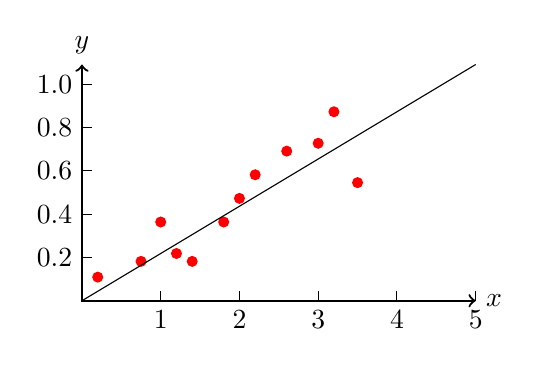
\begin{tikzpicture}
    \pgfmathsetmacro{\ticker}{0.125}
    \draw [<->,thick] (0,3) node (yaxis) [above] {$y$}
            |- (5,0) node (xaxis) [right] {$x$};
    \foreach \i/\texti  in {1,2,3,4,5} {
    \draw (1*\i,0) --(1*\i,\ticker) node[label=below:\texti]{};
    }
    \foreach \j/\textj  in {0.2,0.4,0.6,0.8,1.0} {
    \draw (0,2.75*\j) --(\ticker,2.75*\j) node[label=left:\textj]{};
    }
    \
    \fill[red] (0.2,0.3) circle (2pt);
    \fill[red] (0.75,0.5) circle (2pt);
    \fill[red] (1,1) circle (2pt);
    \fill[red] (1.2,0.6) circle (2pt);
    \fill[red] (1.4,0.5) circle (2pt);
    \fill[red] (1.8,1) circle (2pt);
    \fill[red] (2.0,1.3) circle (2pt);
    \fill[red] (2.2,1.6) circle (2pt);
    \fill[red] (2.6,1.9) circle (2pt);
    \fill[red] (3,2.0) circle (2pt);
    \fill[red] (3.2,2.4) circle (2pt);
    \fill[red] (3.5,1.5) circle (2pt);
    \draw (0,0) -- (5,3) node [] {};
    \end{tikzpicture}
    \caption{根据所给的数据集拟合函数,并根据此函数预测将来的数值}
    \label{Linear_picture}
\end{center}
\end{figure}


如图\ref{Linear_picture}所示,自变量x会与要预测的目标变量y建立一个函数关系。
为了使结果更精确,我们可以指定特定的模型,决定是使用一次函数还是二次函数来更好地贴合数据集,
从而达到更好的预测效果。

在DL4J中,线性回归算法主要有三个部分组成,模型的建立,过程的监听和数据集的构造。
建立模型需要一些超参数。在下面的代码块中指定了一些超参数:第一是随机种子,
由于每次进行神经网络训练时,函数的偏置和权重都是随机的,
我们需要用种子来确保初始情况大致一致,使结果具有可复现性。
第二是OptimizationAlgorithm 和updater,代表了模型的优化算法,
分别决定了学习的方向和学习率的大小。第三是对模型权重的初始化。
第四是对神经元的设置,第六是设置是否进行反向传播。

\begin{figure}[!ht]
\begin{lstlisting}[language=Java]
 MultiLayerConfiguration conf = new NeuralNetConfiguration.Builder()
                .seed(seed)
                .optimizationAlgo(OptimizationAlgorithm.STOCHASTIC_
                GRADIENT_DESCENT)
                .weightInit(WeightInit.XAVIER)
                .updater(new Sgd(learningRate))
                .layer(0, new OutputLayer.Builder(LossFunctions.LossFunction.MSE)
                .backprop(true)
                .build
\end{lstlisting}
\end{figure}

在进行训练的同时我们也要对模型进行监听,
主要用于对函数的损失函数进行监听,从而更好地对算法进行改进。

最后是数据集的构造。我们说过线性回归的数据集包括数据和结果两个部分。
在这里,我们把自变量x称为特征,因变量y称为标签,
首先先创建两个长度为样本数量的数组,分别代表输入和输出数据的数组;
接着根据特征的值随机生成输入和输出的数,最后将其包装成一个类返回给模型,
代码如图\ref{statics_set_creation}所示。

\begin{figure}[!ht]
\begin{lstlisting}[language=Java]
  private static DataSetIterator getTrainingData(int batchSize, Random rand) {
        double [] output = new double[SampleNum];
        double [] input = new double[SampleNum];
        for (int i= 0; i< SampleNum; i++) {
            input[i] = MIN_RANGE + (MAX_RANGE - MIN_RANGE) * rand.nextDouble();
            output[i] = 0.5 * input[i] + 0.1;
        }
        INDArray inputNDArray = Nd4j.create(input, new int[]{nSamples,1});

        INDArray outPut = Nd4j.create(output, new int[]{nSamples, 1});
        DataSet dataSet = new DataSet(inputNDArray, outPut);
        List<DataSet> listDs = dataSet.asList();
        return new ListDataSetIterator(listDs,batchSize);
    }
\end{lstlisting}
\caption{数据集的构造:包括特征和标签}
\label{statics_set_creation}
\end{figure}


当然,这里的线性回归只含有一个自变量和一个因变量,因此被称为一次线性回归或单变量线性回归。
这种模型比较简单,用二维的xy坐标轴即可表示出来。
在实际的操作中还会遇到还有多变量线性回归,在面对更多维度的参数能更好地进行处理。


\subsection{过拟合}
对于机器学习来说,过拟合是一个十分常见的问题。
过拟合具体是指经过机器学习所获得的权重参数,可以拟合训练数据,
却在面对不包含在训练数据中的实际数据时,不能很好的拟合他们。
机器学习的目的就是获得一个更加抽象,以及泛化的模型。
即使是面对未包含在训练数据中的数据,我们也希望能获得较好的拟合结果。
所以我们需要通过一定的方法来抑制过拟合。

过拟合产生的原因,主要有两点:
1.模型具有大量的参数,表现力强
2.训练数据的数量很少


\begin{figure}[!ht]
\begin{center}
\begin{tikzpicture}
    \pgfmathsetmacro{\ticker}{0.125}
    \draw [<->,thick] (-0.5,5) node (yaxis) [above] {$x_2$}
            |- (4,0.4) node (xaxis) [right] {$x_1$};
    \
     \draw[dashed](0,0.7)--(0.2,1.3);
     \draw[dashed](0.2,1.3)--(0.5,1.7);
     \draw[dashed](0.5,1.7)--(0.7,2);
     \draw[dashed](0.7,2)--(0.8,3.2);
     \draw[dashed](0.8,3.2)--(1,3.8);
     \draw[dashed](1,3.8)--(1.3,4.2);
     \draw[dashed](1.3,4.2)--(1.4,4.5);
     \draw[dashed](1.4,4.5)--(1.6,4.6);
     \draw[dashed](1.6,4.6)--(1.8,4.8);
     \draw[dashed](1.8,4.8)--(1.9,4.9);
     \draw[dashed](1.9,4.9)--(2.0,4.92);
     \draw[dashed](2.0,4.92)--(2.1,4.93);
     \draw[dashed](2.1,4.93)--(2.3,4.94);
     \draw[dashed](2.3,4.94)--(2.5,4.95);
     \draw[dashed](2.5,4.95)--(2.8,4.97);
     \draw[dashed](2.8,4.97)--(3,5);
     \draw[gray](0,0.7)--(0.2,1.2);
     \draw[gray](0.2,1.2)--(0.5,1.3);
     \draw[gray](0.5,1.3)--(0.7,1.5);
     \draw[gray](0.7,1.5)--(0.8,2.2);
     \draw[gray](0.8,2.2)--(1,2.8);
     \draw[gray](1,2.8)--(1.3,3);
     \draw[gray](1.3,3)--(1.4,3.2);
     \draw[gray](1.4,3.2)--(1.6,3.3);
     \draw[gray](1.6,3.3)--(1.8,3.4);
     \draw[gray](1.8,3.4)--(1.9,3.42);
     \draw[gray](1.9,3.42)--(2.2,3.43);
     \draw[gray](2.2,3.43)--(2.5,3.46);
     \draw[gray](2.5,3.46)--(2.8,3.48);
     \draw[gray](2.8,3.48)--(3,3.5);
\end{tikzpicture}
\caption{过拟合情况}
\label{over_fitting}
\end{center}
\end{figure}

如图\ref{over_fitting}所示,对于训练用数据来说,大约100个epoch之后,精度便可以达到接近100\%。
但是,对于测试用数据来说,识别精度确只能达到70\%左右,这并非我们所想要的结果。
从上面的分析中可知,模型对训练时没有使用的数据拟合得并不好。

\subsection{正则化}
过拟合作为机器学习中一种常见的问题,自然也有解决的方法。
基于本书主要介绍关于入门方面的知识,在此便不深入介绍。
仅简单介绍一下权值衰减这一方法。

权值衰减是一种常见的用来抑制过拟合的方法。其通过在学习过程在中
对大的权重进行一定比例的惩罚,从而达到过拟合的目的。过拟合往往就是因为
权重参数取值过大才发生的。因此权值衰减不失为一种简单而有效的办法。

实现权值衰减具体方法是为损失函数加上权重的平方范数(L2范数)。
机器学习的目的是减少损失函数的值,使用权值衰减后,
便可以对变大的权重进行惩罚,从而达到抑制的作用。
具体来说,如果将权重记为$\boldsymbol{W}$,L2范数的值便是$\frac{1}{2}\lambda\boldsymbol{W}^2$。
权值衰减便是将L2范数加到损失函数中。在L2范数中,$\lambda$是控制正则化程度的参数。
$\lambda$越大,对数值较大的权重施加的惩罚也就越重。
下面我们用图片来具体解释:

\begin{figure}[!ht]
    \begin{center}
    \begin{tikzpicture}
        \pgfmathsetmacro{\ticker}{0.125}
        \draw [<->,thick] (-0.5,5) node (yaxis) [above] {$x_2$}
                |- (4,0.4) node (xaxis) [right] {$x_1$};
        \
         \draw[dashed](0,0.7)--(0.2,1.3);
         \draw[dashed](0.2,1.3)--(0.5,1.7);
         \draw[dashed](0.5,1.7)--(0.7,2);
         \draw[dashed](0.7,2)--(0.8,3.2);
         \draw[dashed](0.8,3.2)--(1,3.6);
         \draw[dashed](1,3.6)--(1.3,3.8);
         \draw[dashed](1.3,3.8)--(1.4,4);
         \draw[dashed](1.4,4)--(1.6,4.1);
         \draw[dashed](1.6,4.1)--(1.8,4.3);
         \draw[dashed](1.8,4.3)--(1.9,4.4);
         \draw[dashed](1.9,4.4)--(2.0,4.42);
         \draw[dashed](2.0,4.42)--(2.1,4.47);
         \draw[dashed](2.1,4.47)--(2.3,4.43);
         \draw[dashed](2.3,4.43)--(2.5,4.49);
         \draw[dashed](2.5,4.49)--(2.8,4.45);
         \draw[dashed](2.8,4.45)--(3,4.5);
         \draw[gray](0,0.7)--(0.2,1.2);
         \draw[gray](0.2,1.2)--(0.5,1.3);
         \draw[gray](0.5,1.3)--(0.7,1.5);
         \draw[gray](0.7,1.5)--(0.8,2.2);
         \draw[gray](0.8,2.2)--(1,2.8);
         \draw[gray](1,2.8)--(1.3,3);
         \draw[gray](1.3,3)--(1.4,3.2);
         \draw[gray](1.4,3.2)--(1.6,3.3);
         \draw[gray](1.6,3.3)--(1.8,3.4);
         \draw[gray](1.8,3.4)--(1.9,3.42);
         \draw[gray](1.9,3.42)--(2.2,3.43);
         \draw[gray](2.2,3.43)--(2.5,3.46);
         \draw[gray](2.5,3.46)--(2.8,3.48);
         \draw[gray](2.8,3.48)--(3,3.5);
    \end{tikzpicture}
    \caption{权值衰减方法}
    \end{center}
    \end{figure}

如上图所示,测试数据的识别精度没有太大变化。但训练数据和测试数据的识别精度之间的差距
明显缩小了。这证明,过拟合收到了抑制,而训练数据和测试数据的整体识别精度的增加需要依靠其他的
方法,并非权值衰减的作用范围。

\section{逻辑回归}
逻辑回归与线性回归相似,同样用于处理数据的分类问题。
他们的不同之处在于逻辑回归的数据集中只包含数据,神经网络会自我学习,
自行生成一套数据结构模式。在这种模式中,我们只需要提供数据,
不需要提供数据集地的正确答案,其余部分均由神经网络完成对数据的分类。
因此,逻辑回归也被称为无监督学习。

在下图的例子中,我们给出一个数据集(如图\ref{Logic_picture})。
模型并不知道这些数据的意义和用途,只会尝试着找出其中潜藏的数据结构。
在这个例子中,逻辑回归算法会判定这个数据集从属于两个数据簇$a$,$b$,
从而完成数据分类的任务。
\vspace{5pt}

    \begin{figure}[!hb]
    \begin{center}
    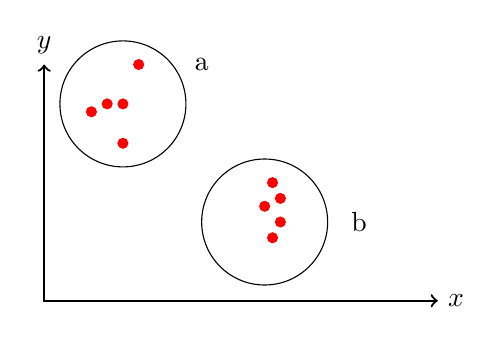
\begin{tikzpicture}
    \draw [<->,thick] (0,3) node (yaxis) [above] {$y$}
        |- (5,0) node (xaxis) [right] {$x$};
    \fill[red] (1,2) circle (2pt);
    \fill[red] (0.6,2.4) circle (2pt);
    \fill[red] (0.8,2.5) circle (2pt);
    \fill[red] (1,2.5) circle (2pt);
    \fill[red] (1.2,3) circle (2pt);
    \node at (2,3) {a};
    \draw  (1,2.5) ellipse (0.8 and 0.8);
    \fill[red] (3,1) circle (2pt);
    \fill[red] (2.8,1.2) circle (2pt);
    \fill[red] (2.9,1.5) circle (2pt);
    \fill[red] (2.9,0.8) circle (2pt);
    \fill[red] (3,1.3) circle (2pt);
    \draw  (2.8,1) ellipse (0.8 and 0.8);
    \node at (4,1) {b};
    \end{tikzpicture}
    \caption{逻辑回归注重数据的分类}
    \label{Logic_picture}
    \end{center}
    \end{figure}


在DL4J中,逻辑回归与线性回归配置类似,主要区别在于神经网络的最后一层输出层:
在线性回归中,最后一个隐藏层是Activation.IDENTITY,即不对数据作处理。
而逻辑回归的最后一层为Activation.SOFTMAX,指定了对当前数据进行分类任务。
代码如下:

\begin{figure}[!hb]
\begin{lstlisting}[language=Java]
        MultiLayerConfiguration conf = new NeuralNetConfiguration.Builder()
        .seed(seed)
        .updater(new Nesterovs(learningRate, 0.9))
        .layer(0, new OutputLayer.Builder(LossFunction.NEGATIVELOGLIKELIHOOD)
                .weightInit(WeightInit.XAVIER)
                .activation(Activation.SOFTMAX)
                .build())
        .build();
\end{lstlisting}
\end{figure}


\section{正向传播}
正向传播也叫前向传播,是指数据从输入层到隐藏层,再到输出层的单向过程。
数据会从输入层输入,经过隐藏层的一层层地变换,最终得出结果数据。
如图\ref{three_layers_picture}是一个典型的三层神经网络,
我们便以此为例解释正向传播。

\begin{figure}[!ht]
    \begin{center}
    \begin{tikzpicture}
    \tikzstyle{arrow} = [thick, ->, >= stealth]
    \tikzstyle{node} = [circle,  minimum width = 1cm, minimum height=1cm ,text centered, draw = black]
    \node[node](I1){$I_1$};
    \node[node, below of = I1, yshift = -1cm](I2){$I_2$};
    \node[node, below of = I2, yshift = -1cm](I3){$I_3$};
    \node[node, right of = I1, xshift = 1.5cm](H1){$H_1$};
    \node[node, right of = I2, xshift = 1.5cm](H2){$H_2$};
    \node[node, right of = I3, xshift = 1.5cm](H3){+1};
    \node[node, right of = H2, xshift = 1.5cm](O1){$O_1$};
    \node[below, below of = I3, yshift = -0.5cm](text1){输入层};
    \node[below, below of = H3, yshift = -0.5cm](text2){隐藏层};
    \node[below, right of = text2, xshift = 1.5cm](text3){输出层};

    \draw[arrow] (I1)--(H1);
    \draw[arrow] (I1)--(H2);
    \draw[arrow] (I2)--(H1);
    \draw[arrow] (I2)--(H2);
    \draw[arrow] (I3)--(H1);
    \draw[arrow] (I3)--(H2);
    \draw[arrow] (H1)--(O1);
    \draw[arrow] (H2)--(O1);
    \draw[arrow] (H3)--(O1);
    \end{tikzpicture}
    \caption{经典的三层神经网络}
    \label{three_layers_picture}
    \end{center}
\end{figure}

隐藏层$H_1$的值由输入层的值和权重所决定,
$W_{(1,1)}$,$W_{(2,1)}$,$W_{(3,1)}$分别代表输入数据$I_1$,$I_2$,$I_3$
对于隐藏层$H_1$的权重。公式如下:

\begin{equation*}
    H_1=I_1W_{(1,1)}+I_2W_{(2,1)}+I_3W_{(3,1)}
\label{Propgate_equation}
\end{equation*}


同理,$H_2$也可表达为相似的公式。经由隐藏层激活函数计算后得到该层的激活值。
同时,输出层的值由隐藏层的值和权值决定,$W_1$,$W_2$分别代表各个隐藏层数据对于
输出层的权重。$b_1$表示偏置,公式如下:

\begin{equation*}
    O_1=H_1W_1+H_2W_2+b_1
    \label{Propgate_output_equation}
\end{equation*}

这样一个由输入层至隐藏层,再由隐藏层至输出层的过程就被称为正向传播。
如图\ref{three_layers_picture}所示,只含有正向传播的神经网络可以用一个有向无环图来表示。
只含有正向传播的神经网络被称为前馈神经网络,
是现今发展较为成熟的一种神经网络。


\section{反向传播}
在正向传播中,神经网络中的数据单向向前传播;因此,我们无法准确知道每一步造成的误差大小,
也无法根据误差对神经网络进行调整更新;反向传播就提供了另一种途径来量化误差并更新权值。
反向传播用于将代价函数最小化,将每一层的误差反向传播给上一层,
由此将误差最小化,如图\ref{back_propagate_picture}。


\begin{figure}[!h]
    \begin{center}
    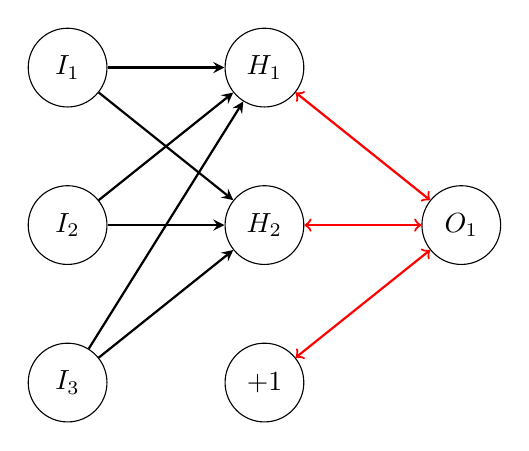
\begin{tikzpicture}
    \tikzstyle{arrow} = [thick, ->, >= stealth]
    \tikzstyle{arrowred} = [thick,<->,red]
    \tikzstyle{node} = [circle,  minimum width = 1cm, minimum height=1cm ,text centered, draw = black]
    \node[node](I1){$I_1$};
    \node[node, below of = I1, yshift = -1cm](I2){$I_2$};
    \node[node, below of = I2, yshift = -1cm](I3){$I_3$};
    \node[node, right of = I1, xshift = 1.5cm](H1){$H_1$};
    \node[node, right of = I2, xshift = 1.5cm](H2){$H_2$};
    \node[node, right of = I3, xshift = 1.5cm](H3){+1};
    \node[node, right of = H2, xshift = 1.5cm](O1){$O_1$};
    \draw[arrow] (I1)--(H1);
    \draw[arrow] (I1)--(H2);
    \draw[arrow] (I2)--(H1);
    \draw[arrow] (I2)--(H2);
    \draw[arrow] (I3)--(H1);
    \draw[arrow] (I3)--(H2);
    \draw[arrowred] (H2)--(O1);
    \draw[arrowred] (H3)--(O1);
    \draw[arrowred] (O1)--(H1);
    \end{tikzpicture}
    \caption{具有反向传播的神经网络}
    \label{back_propagate_picture}
    \end{center}
\end{figure}


为了计算每一层神经元所产生的误差,我们引入$\delta_{j}^{(l)}$,
代表第l层的第j个节点所产生的误差。
由此可得最后一层输出层的误差公式为$\delta_{j}^{(3)}=a_{j}^{(3)}-y_{j}$,其中$a_{j}^{(3)}$
代表神经网络计算出的值,而$y_{j}$代表数据对应的真实值。

误差向前一层传播时,公式需更改为
$\delta^{(2)}=(\Theta^{(2)})^{T}\delta^{(3)}*g'(z^{(2)})$,$(\Theta^{(n)})^T$代表
第n层代价函数的转置,$z^{(n)}$等于$\Theta^{(n-1)} a^{(n-1)}$,最后
$g(z)$代表该层的激活函数。依据这个公式,我们就而可以将误差逐层上传,并实现对神经网络
参数的修改。

反向传播实际上与正向传播很相似。他们的计算方法类似,区别在于正向传播是从前向后计算,
而反向传播是从后向前计算。其实,$\delta_{j}^{(l)}$即是
该层代价函数关于该层对应的所有输入单元加权和的偏导。以图\ref{back_propagate_picture}为例,$\delta_{1}^{(3)}$可表达为
$\delta_{1}^{(3)}=\frac{\partial}{\partial z_{1}^{(3)}} \operatorname{cost}(\mathrm{i})$,
其中$cost(i)$代表该层的代价函数,
$z_{1}^{(3)}$等于$a_{1}^{(2)}*W_{(1,2)}+a_{2}^{(2)}*W_{(2,2)}$。
$\delta_{j}^{(l)}$衡量了神经网络计算中的中间值,代表了神经网络权重改变的程度大小,
使我们对整个网络有更深入的了解。

反向传播只是正向传播的逆向过程。我们还是以图\ref{back_propagate_picture}为例,
由上可知$\delta_{1}^{(3)}=a_{1}^{(3)}-y_{1}$,而逆向到$\delta_{2}^{(2)}$的算式
可表达为$\delta_{2}^{(2)}=(W_{(2,2)})^{-1}*\delta_{1}^{(3)}$。这样的逆过程与
正向传播的计算过程区别不大;所以说,反向传播与正向传播在形式和计算方法上都很相似。

反向传播广泛地应用于循环神经网络,例如机器翻译、语言理解等前沿应用。
这种结构的网络往往存在记忆单元和注意力机制,要求复杂的求导计算,
例如Google语音助手的上下文理解功能。反向传播促进了记忆神经网络的发展,
目前正在探索和发展中。



\section{全连接网络}
全连接层网络(MLP,Multilayer Perceptron)又叫多层感知机,
特点是上一层的所有神经元都与下一层的所有神经元相连接,因此又叫全连接层。
如图\ref{three_layers_picture}就是一个简单的全连接层,最底层是输入层,中间是隐藏层,最后是输出层。
在计算第n层的某个节点的时候,输入的参数是第n-1层的所有节点的加权。

从图\ref{multilayer_perceptron}可以看出,全连接网络的所有参数就是各个层的权重和偏置。
确定并最优化这些参数就是一个最优化的问题,最简单的就是利用梯度下降(SGD),
首先随机初始化所有参数,然后进行迭代训练,不断地更新梯度和参数,
直到满足某个条件为止。全连接网络应用广泛,例如MNIST手写数字识别等。

\begin{figure}[!ht]
    \begin{center}
    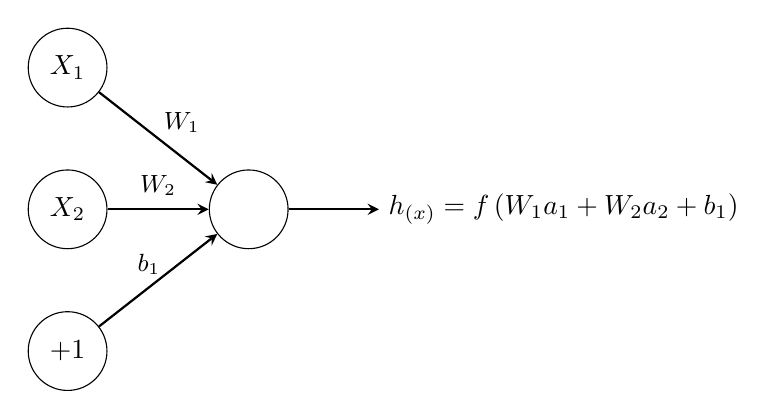
\begin{tikzpicture}
    \tikzstyle{arrow} = [thick, ->, >= stealth]
    \tikzstyle{node} = [circle,  minimum width = 1cm, minimum height=1cm ,text centered, draw = black]
    \node[node](X1){$X_1$};
    \node[node, below of = X1, yshift = -0.8cm](X2){$X_2$};
    \node[node, below of = X2, yshift = -0.8cm](+1){+1};
    \node[node, right of = X2, xshift = 1.3cm](Output){};
    \node[right of = Output, xshift = 3cm](Output1){$h_{(x)}=f\left(W_1 a_1+W_2 a_2+b_1\right)$};

    \draw[arrow](X1)--(Output);
    \draw[arrow](X2)--(Output);
    \draw[arrow](+1)--(Output);
    \draw[arrow](Output)--(Output1);

    \coordinate[label = left:{\small $W_1$}]() at(1.8, -0.7);
    \coordinate[label = left:{\small $W_2$}]() at(1.5, -1.5);
    \coordinate[label = left:{\small $b_1$}]() at(1.3, -2.5);

    \end{tikzpicture}
    \caption{全连接层中的一个节点}
    \label{multilayer_perceptron}
    \end{center}
\end{figure}




\chapter{有监督学习}
\label{chap:supervised}
机器学习分为:监督学习,无监督学习。
本章先介绍\emph{监督学习}(supervised learning),
它从给定的训练数据集中学习出一个函数,用于对新数据的预测。
监督学习的训练集包括输入和输出,也即是特征和目标。
训练集中的目标是由人标注的,利用这些已知数据和其输出训练得到一个最优模型(目标函数)。
监督学习是训练神经网络和决策树的常见方法。
最典型的算法是KNN和SVM,用于回归分析和统计分类。

\section{训练过程}
有监督学习最常见的就是:回归(Regression)和分类(Classification)。
一般来说,定量输出称为回归,或是对连续变量预测;
定性输出称为分类,就是对离散变量进行预测。K-近邻(KNN)是一种分类算法,
而之前提到的线性回归,就是利用已知数据集求线性函数,使其尽可能地拟合数据,
也就是让损失函数最小。

\section{回归问题}
回归分析分为:线性回归、逻辑回归(Logistic Regression)。
实际上,逻辑回归就是对线性回归的输出又进行了一次特殊函数的处理,
使其输出一个分类可能性的概率,这个特殊的函数通常是sigmoid函数:
$$ y = \frac{1}{1+e^{-x}} $$
\begin{figure}[!htbp]
\centering
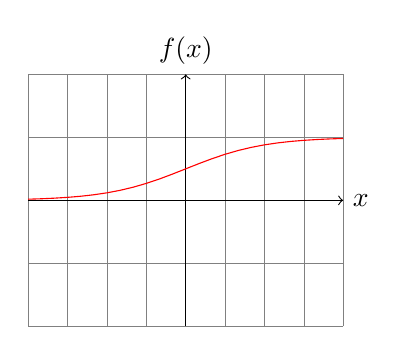
\begin{tikzpicture}[yscale=0.8, xscale=0.5]
  \draw[very thin,color=gray] (-4,-2) grid (4,2);
  \draw[->] (-4,0) -- (4,0) node[right] {$x$};
  \draw[->] (0,-2) -- (0,2) node[above] {$f(x)$};
	\draw[color=red, domain=-4:4] plot (\x,{1/(1+e^-\x)});
\end{tikzpicture}
\end{figure}

Sigmoid函数是机器学习非常重要的一个函数,
当$x>0$时,Sigmoid函数大于0.5;当$x<0$时,Sigmoid函数小于0.5。
因此,把拟合曲线的函数值带入Sigmoid函数,
比较$f(x)$与0.5的大小就可判断其分类。
总的来说,Sigmoid函数具有以下几个良好性质:
\begin{enumerate}
	\item 单调可微,具有对称性。
	\item 便于求导。
	\item 定义域为$[-\infty, +\infty]$,值域为$(0, 1)$,可将任意值映射为概率。
\end{enumerate}

\subsection{线性回归}
之前章节介绍过线性回归的数学模型,并尝试用梯度下降法,找到线性函数的参数,来拟合数据集。
所以实现线性回归的代码,得首先实现梯度的算法函数,分为:SGB、BGD和MBGD。

因为\emph{批梯度下降}是使用所有的数据样本拟合出来的假设函数,
所以计算梯度也就会涉及到所有的样本数据,这种情况就是所谓的BGD(Batch Gradient Descent)。
结合最小二乘法的定义,定义损失函数
$J(\theta)=\frac{1}{2}\sum_i^m(y_i-h_\theta(x^i))^2$
现在问题就转化为求解最优的$\theta$,使损失函数$J(\theta)$取最小值。

$$ \theta_j:=\theta_j-\alpha\frac{\delta}{\delta\theta_j}J(\theta) $$

我们先随便给$\theta$一个初始化的值(多默认为1),然后改变$\theta$值让J($\theta$)的取值变小,
不断重复改变$\theta$使$J(\theta)$变小的过程直至$J(\theta)$约等于最小值。
此算法也称为\emph{最小均方算法}(Least mean square,LMS算法)。
$$ \theta_j:=\theta_j+\frac{1}{\alpha}\sum_i^m (y_i-h_\theta(x^i))x^i_j $$
\noindent
使用伪代码表示如下,:
\begin{lstlisting}[escapeinside=``]
repeat{    
	`$ \theta_j:=\theta_j+\frac{1}{\alpha}\sum_i^m (y_i-h_\theta(x^i))x^i_j $`
  for every j=0, ... , n)
}
\end{lstlisting}

\noindent
其中$\alpha$称为步长(learning rate),控制$\theta$每次向$J(\theta)$变小的方向迭代的幅度。
由以上伪代码,也容易发现BGD(\emph{批梯度下降})每次迭代都得把所有样本计算一次,计算量很大。
把整个过程分解一下,包含:初始化、求偏导和梯度下降。
\vspace{0.3cm}

\noindent
Java代码,大致如下。
\begin{lstlisting}[language=Java, escapeinside=``]
	// `$h(x) = \theta_0 * x_0 + \theta_1* x_1 + \theta_2 * x_2$`
	public class LinearRegression {
		public LinearRegression(double[][] data,double alpha,int iteration){}

		private void     initialize_theta(){}
		public  void     train(){}
		private double[] partial_derivative(){}
		private double   partial_derivative_of_theta(int j){}
		private double   h_theta_x_i_minus_y_i_times_x_j_i(int i,int j){}
	}
\end{lstlisting}



\subsection{逻辑回归}
Sigmoid的其中一个优点就是容易求解导数,利于编码实现。
推导过程略,相应的实现代码如下:
$$ y = \frac{1}{1+e^{-x}}, y' = y*(1-y) $$

\begin{lstlisting}[language=Java]
	public static double sigMoid(double value) {
		double e_x = Math.pow(Math.E, -value);
		double result = 1 / (1 + e_x);
		return result;
	}

  public static double sigMoidDerivative(double value) {
		double A = sigMoid(value);
		double B = 1 - sigMoid(value);
		double result = A * B;
		return result;
  }
\end{lstlisting}


\section{SVM}
在机器学习章节中,我们提到过利用SVM(支持向量机)作为数据分类的一种方法,并提到了
SVM的实质其实就是正确分类数据的直线,并且分类直线与支持向量的间隔较远。在这样的基础
上,我们有必要对坐标系内点与直线的距离进行研究。假设$\mathbf{w_{i}}$为分类直线
的函数,$\delta_{i}$代表坐标与分类直线的距离,$\mathbf{\|\mathbf{w}\|}$代表向量
$\mathbf{w}$的范数\footnote{范数是对向量长度的度量,如果一个向量可以表示为
$\mathrm{W}=(w_1, w_2, w_3, \ldots ,w_n)$,那么该向量的范数则为
$\|w\|_{n}=\sqrt[n]{m_{1}^{p}+m_{2}^{n}+...+w_{n}^{n}}$},由此我们可以得到一般性的点到直线距离公式:

\begin{equation}
	\boldsymbol{\delta}_{i}=\frac{1}{\|\mathbf{w}\|}\left|g\left(x_{i}\right)\right|
\end{equation}

在二维坐标中,利用解析几何的知识,我们可以将公式简化为更容易理解的形式:
$D=(Ax+By+c) / \sqrt{A^{2}+B^{2}}$,
其中$Ax+By+c$就相当于$g(x_{i})$,$\sqrt{A^{2}+B^{2}}$相当于$\mathbf{w}$的范数。
这个公式的代码实现如下:
$$ ax + by + c = 0 $$

\begin{lstlisting}[language=Java]
	public double getDistance(double x, double y){
        double denominator = a * x + b * y + c;
        double numerator = Math.sqrt(a * a + b * b);
        double result = denominator / numerator;
        return result;
    }
\end{lstlisting}

在界定了分隔直线后,空间就被分成了$g(x_{i}) > 0$和$g(x_{i}) < 0$
两个部分,以此便可以判断数据类型的不同。与此同时,根据我们在机器学习章节
中提出的要求,最佳直线应该与所有支持向量等距且最远;因此,我们我们需要对最佳
直线与支持向量间的距离进行研究。

\begin{figure}[!ht]
    \begin{center}
    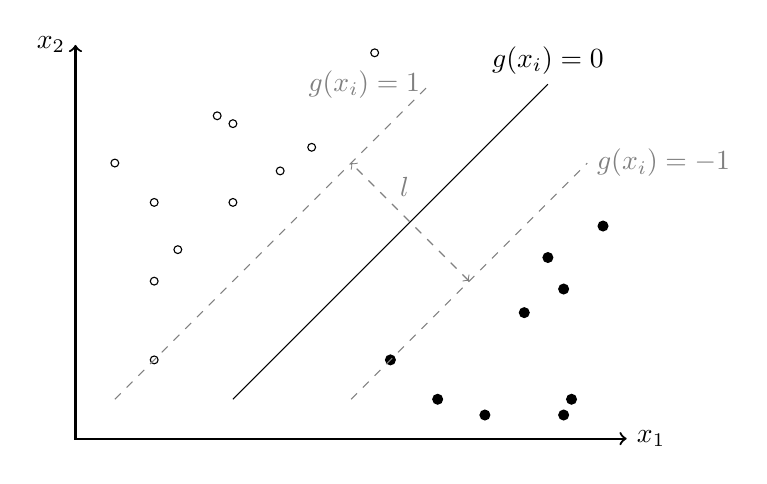
\begin{tikzpicture}
        \pgfmathsetmacro{\ticker}{0.125}
        \draw [<->,thick] (0,5) node (yaxis) [left] {$x_2$}
				|- (7,0) node (xaxis) [right] {$x_1$};
		\node[draw,circle,inner sep =1pt] (A) at (1,3) {};
		\node[draw,circle,inner sep =1pt] (B) at (0.5,3.5) {}; 
		\node[draw,circle,inner sep =1pt] (C) at (1,2) {}; 
		\node[draw,circle,inner sep =1pt] (D) at (1,1) {}; 
		\node[draw,circle,inner sep =1pt] (E) at (2,4) {};
		\node[draw,circle,inner sep =1pt] (F) at (2,3) {};
		\node[draw,circle,inner sep =1pt] (G) at (1.3,2.4) {};
		\node[draw,circle,inner sep =1pt] (H) at (3,3.7) {};
		\node[draw,circle,inner sep =1pt] (I) at (3.8,4.9) {};
		\node[draw,circle,inner sep =1pt] (J) at (2.6,3.4) {};
		\node[draw,circle,inner sep =1pt] (K) at (1.8,4.1) {};
		\fill[black] (4,1) circle (2pt);
		\fill[black] (4.6,0.5) circle (2pt);
		\fill[black] (5.2,0.3) circle (2pt);
		\fill[black] (5.7,1.6) circle (2pt);
		\fill[black] (6,2.3) circle (2pt);
		\fill[black] (6.2,1.9) circle (2pt);
		\fill[black] (6.7,2.7) circle (2pt);
		\fill[black] (6.3,0.5) circle (2pt);
		\fill[black] (6.2,0.3) circle (2pt);
		\draw[dashed, color=gray, domain=0.5:4.5]    plot (\x,{1 * \x}) node[left]{$g(x_{i}) = 1$};
		\draw[color=black, domain=2:6]    plot (\x,{1 * \x - 1.5}) node[above]{$g(x_{i}) = 0$};
		\draw[dashed, color=gray, domain=3.5:6.5]    plot (\x,{1 * \x - 3}) node[right]{$g(x_{i}) = -1$};
		\draw[dashed, color=gray, <->] (5,2)--(3.5,3.5) node[right] at (4, 3.2){$l$};
        \end{tikzpicture}
		\label{SVM_supersurface_picture}
		\caption{二维向量的线性分类器}
    \end{center}
\end{figure}

在这里,我们构建了名为“线性分类器”的模型来解决这一问题,如图\ref{SVM_supersurface_picture}。
这个问题的关键在于比较支持向量与分类直线的距离,那么我们不妨设当$g(x_{i}) > 0$
时,直线上方的支持向量经过直线$g(x_{i}) = 1$;同理,$g(x_{i}) < 0$时,直线下方
的支持向量经过直线$g(x_{i}) = -1$,这样假设方便我们进行进一步的处理。我们可以得出
$g(x_{i}) = 1$和$g(x_{i}) = -1$间的距离,即$l = 2 /\|w\|$。同时,SVM的目标是在对数据进行
正确分类的情况下,最大化分类直线和支持向量的距离;由此,我们可以得到以下关系:

$$y_{i}\left(w x_{i}-b\right)>=1$$
$$\max(2 /\|w\|)$$

可以看到最大化$2 / \|w\|$,也就是最小化$\|w\|$;同时,利用高等数学的知识,我们能对其
进行等价转化,这样就得到了SVM的基本形式:

$$y_{i}\left(w x_{i}-b\right)>=1$$
$$\min \frac{1}{2}\|w\|^{2}$$

最后,通过拉格朗日对偶,我们能够将上面的式子进一步转化为拉格朗日对偶性问题。在这个问题中
我们通过添加拉格朗日乘子$\alpha_{i} \geq 0$,写出拉格朗日函数和对应的目标函数:

$$L(w, b, \alpha)=\frac{1}{2}\|w\|^{2}-\sum_{i=1}^{n} \alpha_{i}\left(y_{i}\left(w x_{i}-b\right)-1\right)$$
$$\min _{w, b} \max _{\alpha \geq 0} L(w, b, \alpha)$$

在实际的SVM应用中,向量的维度往往不止二维,会出现三维甚至更多维度。线性函数在不同维度的空间中
有不同的形式,例如在一维空间中是一个点,二维空间中是一条直线,三维空间是一个平面,如果不关注
维数,线性函数又统称为超平面;此时我们研究函数的工具可能有变化,但线性分类器的基本思路仍然
不变。我们依然可以通过基本形式和拉格朗日函数进行求解,这种方法具有普遍性。


\section{卷积神经网络}
卷积神经网络(Convolutional Neural Network,简称CNN)属于前馈神经网络。与全连接
神经网络不同,卷积神经网络只会计算上一层神经网络的部分单元,而全连接网络会计算所有单元。
在大型图像处理上,卷积神经网络具有极大的优势;以常见的图像识别为例,神经网络的输入
就是图像中的各个像素点,全连接网络的做法是将所有像素点不加以区分地全部输入下一层计算;
然而图像识别的关键在于找到图像中的相邻或成群的像素点集,从而找到图像中各部分的“边缘”,
全连接网络囫囵吞枣的做法显然效率不高。卷积神经网络则利用滤波器(Fliter)预先将图像中相邻
像素之间的“边缘”过滤出来,从而大大提高了效率。

\subsection{卷积层}
\subsection{池化层}
\subsection{全连接层}
\subsection{LeNet}
\section{手写识别示例}

\chapter{无监督学习}
\label{chap:unsupervised}
机器学习主要分为三类:监督学习(supervised Learning)、增强学习(reinforcement learning)、无监督学习(unsupervised
learning)。也存在半监督学习(semi-supervised learning)这种情况,但在此不予讨论。

简单来说,区分监督学习和无监督学习的方法就是输入数据是否有标签(label)。
如若没有标签则为无监督学习。
我们以机器学习中的分类(classfication)算法来举例,
对于分类算法来说,输入的训练数据有特征(feature),有标签(label)。
所谓的学习,其本质就是找到特征和标签间的关系(mapping)。
而去判断一个分类算法的成功与否的方法,便是当我们输入有特征无标签的未知数据时,
能否通过已知关系(参数)得到未知数据标签。

举个简单的例子,有监督学习相当于刷算法题的时候你知道答案,
而无监督学习相当于你根本就没有答案,只能靠自己摸索。
所以,与我们的常识相符,无监督学习的准确度往往比起有监督学习要低得多。
那也许你会问了,既然无监督学习准确度那么低,为什么我们还要用它呢?
那是因为在实际情况下,标签的获取需要极大的人工量,还不能保证变迁的准确性。
所以,无监督学习也是十分重要的。

\section{聚类算法}
聚类是数据挖掘中的概念,其定义为按照某个标准把一个数据集分隔成不同的类或簇,
使得相同类里的数据相似程度尽可能大。反之,不在同一个类里的数据,
其差异也要尽可能大。“物以类聚,人以群分”就能大概指代聚类算法的意思。

讲到这里,我们需要区分聚类(clustering)与分类(classification)之间的区别。
对于聚类来说,我们在聚类时,并不关心其中某一类是什么,我们需要实现的目标只是把
相似的东西分到一起。因此,对于聚类算法来说,只要知道相似度衡量的标准就可以开始训练了。
与之相对的,分类算法需要你告知它,它需要将数据分成哪些具体的类别,
所以分类算法需要从训练集中进行学习,从而明白如何对未知数据进行分类。
这就是聚类和分类的区别。

聚类的步骤主要如下:
1.数据准备:将数据转换为标准输入形式,使用特征标准化等方法;
2.特征选择:从最初的特征中选择最有效的特征,并将其存储于向量中;
3.特征提取:通过对所选择的特征进行转换,得到新的重点特征;
4.聚类:首先选择合适特征类型的某种距离函数进行接近程度的度量,而后执行聚类或分组;
5.聚类结果评估:对聚类结果进行评估,评估主要分为3种:外部有效性评估、内部有效性评估和相关性测试评估。

聚类主要分为层次化聚类算法,划分式聚类算法,基于密度的聚类算法,基于网格的聚类算法,基于模型的聚类算法等。
下面我们就挑出几个重要的算法为大家进行讲解。

\subsection{K-means算法}
K-Means算法的特点是类别的个数是人为给定的,
其假设数据之间的相似度可以使用欧氏距离度量,
如果不能使用欧氏距离度量,要先把数据转换到能用欧氏距离度量。

接下来,我们简单介绍一下流程:
首先,我们有在n维向量当中的一堆点,这里以二维空间为例。

%图片

接着我们随机生成k个聚类中心点,相当于将其分为几个类别。
然后分别计算每一个数据点到这些中心的距离,把距离最短的那个当成自己的类别。
这样就可以发现每个点都已经被分类了(有一个中心点),但是并不准确。

%图片

接下来就是无监督学习,使得分类变得更加准确的时候。
我们一开始随机确定的分类点,这时候就要变化了。
而它变化的标准就是“收复”附近的点,所以它将往所有它这一类别的点的坐标平均值移动,
也就是移向中心。而到达中心后,将再一次判断各个点到k个中心点的距离,
选取离每个点最近的中心点作为它的类别,以此类推。

%图片

伪代码流程如下所示:
\begin{lstlisting}[language=Java]
public static double K-Means(输入数据,中心点个数K){
    获取输入数据的维度Dim和个数N
    随机生成K个Dim维的点
    while(算法未收敛){
        对N个点:计算每个点属于哪一类。
        对于K个中心点:
            1,找出所有属于自己这一类的所有数据点
            2,把自己的坐标修改为这些数据点的中心点坐标
    }
    return 结果
}
\end{lstlisting}

接下来,我们来说明一下k-means算法使用过程中有可能会遇到的问题。
1.测量距离的方法
并非一定要使用欧氏空间这个方法,只需满足以下条件都可以用:
首先有个分类两个点的方法的算符记作$$<\vec{a}, \vec{b}>$$,
并且其具有交换性$<\vec{a}, \vec{b}>=<\vec{b}, \vec{a}>$。
其次需要可以求一堆点的平均值的算法(求中心点):
$\vec{\mu}=\operatorname{Mean}\left(\overrightarrow{a_{1}}, \ldots, \overrightarrow{a_{n}}\right)$
求出后只需满足:$\sum_{i=1}^{n}\left(\vec{\mu}-\overrightarrow{a_{i}}\right)^{2}$。

2.如何知道是否收敛?
使用代价函数:$\tilde{J}=\sum_{i=1}^{C} \sum_{j=1}^{N} r_{i j} \times \nu\left(x_{j}, \mu_{i}\right)$。
其中:$\nu\left(x_{j}, \mu_{i}\right)=\left\|x_{j}-\mu_{i}\right\|^{2}$。
代价函数的差分值小于一定数值的时候(N次越不过最小值点)即可认为是收敛了。

3.代价函数不收敛,怎么办?
首先说一下什么时候容易发生震荡:
在数据点个数比较少而且比较稀疏的时候容易发生这种事情,发生的原因大约有两种常见的:
1、陷入某个环里,然后开始震荡,它将会绕着中心点进行低频振荡。
2、两个点互相交换,每次交换不改变J的值就收敛了,
如果交换以后不幸影响了其它的点,就出现了高频振荡。
这个时候给出一种简单的解决方案:阻尼。
简而言之,就是更新自己位置的时候考虑一下原来的位置,
一般阻尼比(在0~1之间取值)决定收敛速度,收敛的慢了也就不容易震荡,
也就越容易陷入局部极小值,也就是说,不震荡的情况下我们应该把阻尼比尽可能取小一点
$\vec{C}^{u p d}=\vec{C}^{n e w} \times(1-\xi)+\vec{C}^{o l d} \times \xi$
$\vec{C}^{u p d}$是最后中心点的取值,$\vec{C}^{n e w}$是当前集合的中心点,
$\vec{C}^{o l d}$是原来的中心点坐标。

\subsection{DBScan算法}

\section{DL4J示例}
\chapter{神经网络}
\label{chap:neuralnetwork}

\section{评价标准}
准确率、召回率、精准率
\chapter{深度学习}
\label{chap:deeplearning}

由神经元提出的感知机模型,只适用于解决二分类问题,对于多分类却无能为力,
而多层感知机却能解决这个问题。

\begin{figure}[!htb]
	\centerline{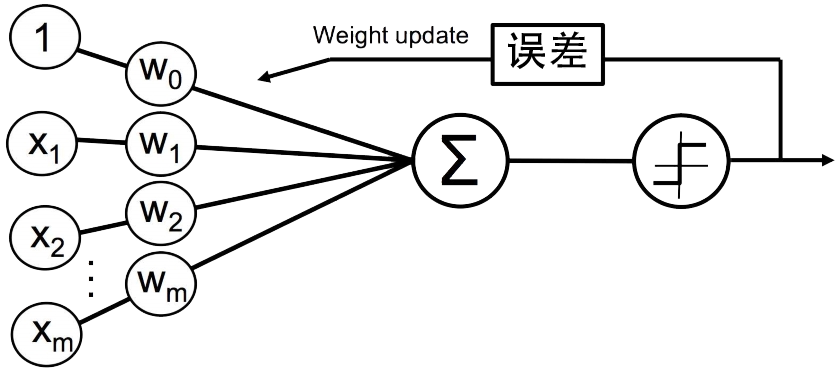
\includegraphics[width=.25\figwidth]{images/perceptron.png}}
	\label{fig:part2_perceptron}
	\caption{感知机}
\end{figure}

\noindent
我们知道感知机可以实现AND、OR、NAND逻辑,而XOR正好可以由它们推算得出:
$x1\;\oplus\;x2 = (x1\;|\;x2)\;\&\;(x1\;\bar{\&}\;x2)$

\begin{figure}[!htb]
	\centerline{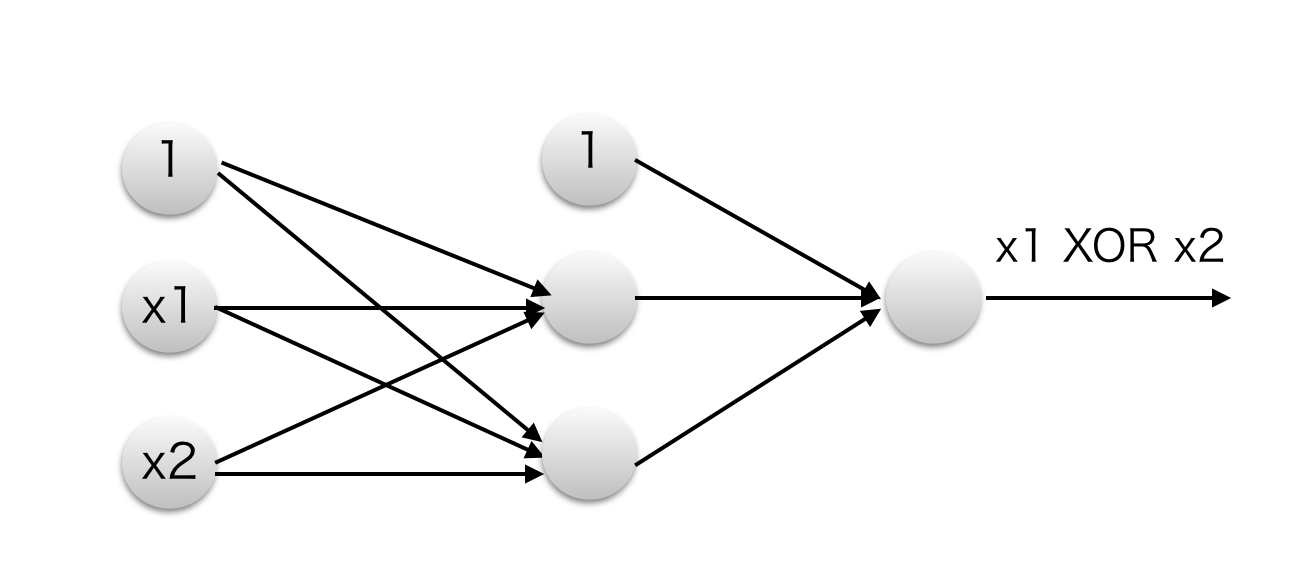
\includegraphics[width=.25\figwidth]{images/xor.png}}
	\label{fig:part2_xor}
	\caption{异或}
\end{figure}

\noindent
这就是深度学习的魅力,但为什么在感知机提出来之后却停滞发展二十年呢?
对于普通的二分类问题,使用的损失函数是基于点线距离的,但毕竟不是一个通用的解决方案。
用于解决多分类问题的时候,就会显得非常笨重,越来越不好用。
实际上,感知机和SVM非常相似,主要差别在于超平面(分割线)是否唯一,是否满足间隔最大化。
感知机是不要求间隔最大的,只要能分开数据就算解决了。

\section{多层感知机}
本节以XOR为例,作为深度学习的入门铺垫。
已知,单层感知机是可以实现AND、OR、NAND逻辑功能的。
如下图:


\begin{figure}[!htb] \centering 
	\begin{tikzpicture}
		\node at (0,0) {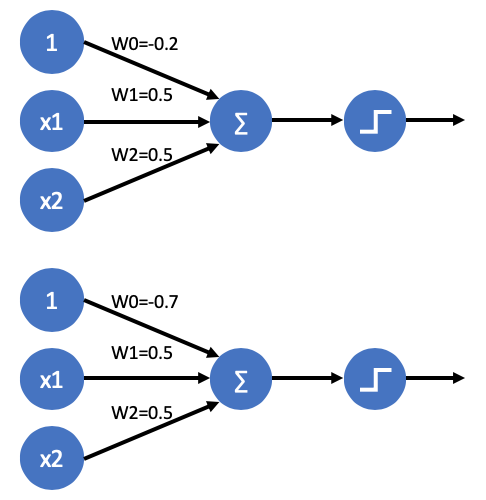
\includegraphics[width=6cm]{images/perceptron_and_or.png}};
		\node at (4,1.6) {逻辑OR};
		\node at (5.5,1) {\small{\(1,0\)=>真,\(1,1\)=>真,\(0,0\)=>假}};
		\node at (4,-1.6) {逻辑AND};
		\node at (5.5,-2.2) {\small{\(1,0\)=>假,\(1,1\)=>真,\(0,0\)=>假}};
	\end{tikzpicture}
	\caption{感知机模型:AND、OR}
\end{figure}

\noindent
感知机的参数如上,我们定义了AND和OR的运算模型,而NAND是AND相反运算,
只要把上图AND的参数都取反即可:$(0.5, 0.5, 0.7) \Rightarrow (-0.5, -0.5, 0.7)$。
示意图,如下。
\begin{figure}[!htb]
	\centerline{
\includegraphics[width=.25\figwidth]{images/xor_or_nand.png}}
	\label{fig:part2_xor_or_nand}
	\caption{多层感知机求解异或}
\end{figure}

\noindent
感知机的最大缺点是误差计算是基于经验的(点到直线距离),而不是基于输出结果。
如果误差的调节,能反应到$w$和$b$,势必要求整个调整过程是可微的,也就是一个平滑的过程。
这个平滑的调节就是基于偏导数实现的,也就是梯度。
因此,这也要求从输入到输出,从误差到输入是一个可以微调的平滑过程,这样才有利于机器学习。
实际上,这就是一个迭代求极值点的过程,直到误差最小或者迭代次数到达。
所谓的前向传播和反向传播,就是这个道理。


\begin{figure}[!htbp]
	\centering
	\begin{minipage}{0.33\textwidth}
	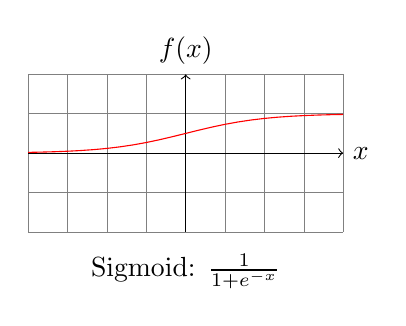
\begin{tikzpicture}[scale=0.5]
		\draw[very thin,color=gray] (-4,-2) grid (4,2);
		\draw[->] (-4,0) -- (4,0) node[right] {$x$};
		\draw[->] (0,-2) -- (0,2) node[above] {$f(x)$};
		\draw[color=red, domain=-4:4] plot (\x,{1/(1+e^-\x)});
		\node at (0, -3) {Sigmoid: $\frac{1}{1+e^{-x}}$};
	\end{tikzpicture}
	\end{minipage}%
	\begin{minipage}{0.33\textwidth}
	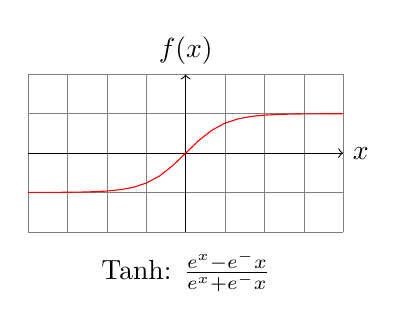
\begin{tikzpicture}[scale=0.5]
		\draw[very thin,color=gray] (-4,-2) grid (4,2);
		\draw[->] (-4,0) -- (4,0) node[right] {$x$};
		\draw[->] (0,-2) -- (0,2) node[above] {$f(x)$};
		\draw[color=red, domain=-4:4] plot (\x,{(e^\x-e^-\x)/(e^\x+e^-\x)});
		\node at (0, -3) {Tanh: $\frac{e^x-e^-x}{e^x+e^-x}$};
	\end{tikzpicture}
	\end{minipage}%
	\begin{minipage}{0.33\textwidth}
		\vspace{0.55cm}
		\begin{tikzpicture}[scale=0.5]
			\draw[very thin,color=gray] (-4,-2) grid (4,2);
			\draw[->] (-4,0) -- (4,0) node[right] {$x$};
			\draw[->] (0,-2) -- (0,2) node[above] {$f(x)$};
			\draw[color=red, domain=-4:0] plot (\x,0);
			\draw[color=red, domain=0:2] plot (\x,\x);
		\node at (0, -3.2) {ReLu: 
				$\begin{cases} 
					x&\text{x>=0}\\0&\text{x<0}
				\end{cases}$};
		\end{tikzpicture}
	\end{minipage}%
\end{figure}

感知机的缺点来源于激活函数是阶跃函数$Sign$,它不是连续可导的函数,无法微调误差。
换成$ReLu, Simoid, TanH$就可以让感知机重获新生。
输出结果不再是$0$和$1$而是$(0,1)$之间的概率值,代表更应该是哪个结果。

\section{PlayGround}
PlayGround是一个在线演示神经网络的平台,是一个入门神经网络非常直观的网站。
它图形化地展示神经网络的训练过程,非常有利于初学者获得感性认识。
PlayGround演示页面由
DATA(数据)、FEATURES(特征)、HIDDEN LAYERS(隐含层)、OUTPUT(输出层),
四个部分组成。

在DATA一栏里提供了4种不同形态的数据,分别是圆形、异或、高斯和螺旋。
还可以对这些数据进行配置:噪声、训测比、批大小(Batch)。
平面内的数据分为蓝色和黄色两种。





